\documentclass[serif,mathserif,final]{beamer}
\mode<presentation>{\usetheme{Lankton}}
\usepackage{amsmath,amsfonts,amssymb,breqn,times,pxfonts,xspace}
\usepackage{graphicx}
\usepackage{color}
\usepackage{wrapfig}
\graphicspath{{../figures/}}
\usepackage[orientation=landscape,size=custom,width=140,height=70,scale=1.4,debug]{beamerposter}

%%%%%%%%%%%%%%%%%%%%%%%%%%%%%%%%%%%%%%%%%%%%%%%%%%%%%%%%%%%%%%%%%%%%%
% Macros
%%%%%%%%%%%%%%%%%%%%%%%%%%%%%%%%%%%%%%%%%%%%%%%%%%%%%%%%%%%%%%%%%%%%%
\newcommand\seteq{\mathrel{\overset{\makebox[0pt]{\mbox{\normalfont\tiny\sffamily set}}}{=}}} % equality with the text "set"
\newcommand\bbR{\ensuremath{\mathbb{R}}} % Real numbers
\newcommand\bbZ{\ensuremath{\mathbb{Z}}} % Integers
\newcommand\bbE{\ensuremath{\mathbb{E}}} % Expectation
\DeclareMathOperator*{\tr}{tr} % Trace
\DeclareMathOperator*{\diag}{diag} % Diagonal matrix
\DeclareMathOperator*{\sign}{sign} % Sign
\DeclareMathOperator*{\var}{Var} % Variance
\DeclareMathOperator*{\cov}{Cov} % Covariance
\newcommand{\1}{\mathbb{I}} % Indicator
\DeclareMathOperator*{\argmax}{arg\,max} % argmax
\DeclareMathOperator*{\argmin}{arg\,min} % argmin
\DeclareMathOperator*{\minimize}{minimize} % minimize
\DeclareMathOperator*{\maximize}{maximize} % maximize

%%%%%%%%%%%%%%%%%%%%%%%%%%%%%%%%%%%%%%%%%%%%%%%%%%%%%%%%%%%%%%%%%%%%%
% Custom Beamer Setting
%%%%%%%%%%%%%%%%%%%%%%%%%%%%%%%%%%%%%%%%%%%%%%%%%%%%%%%%%%%%%%%%%%%%%
\setbeamertemplate{caption}[numbered]
\setbeamertemplate{itemize/enumerate body begin}{\normalfont}
\setbeamertemplate{itemize/enumerate subbody begin}{\normalfont}
\setbeamertemplate{itemize/enumerate subsubbody begin}{\normalfont}
\setbeamertemplate{bibliography item}[numbered]

%-- Header and footer information ----------------------------------
\newcommand{\footleft}{}
\newcommand{\footright}{Christopher B. Choy\textsuperscript{\dag}, Michael
  Stark\textsuperscript{\ddag}, Sam Corbett-Davies\textsuperscript{\dag},
  Silvio Savarese\textsuperscript{\dag}}
\title{Enriching Object Detection with 2D-3D Registration and Continuous
  Viewpoint Estimation}
\author{Christopher B. Choy\textsuperscript{\dag}, Michael
  Stark\textsuperscript{\ddag}, Sam Corbett-Davies\textsuperscript{\dag},
  Silvio Savarese\textsuperscript{\dag}}
\institute{\textsuperscript{\dag}Stanford University,
  \textsuperscript{\ddag}Max Planck Institute for Informatics}
%-------------------------------------------------------------------

%-- Main Document --------------------------------------------------
\begin{document}
\begin{frame}{}
  \begin{columns}[t]

    %-----------------------------------------------------
    % Column 1 
    %-----------------------------------------------------
    \begin{column}{0.24\linewidth}


      %-- Block 1-1 --------------------------------------
      \begin{block}{Motivation}
        \begin{itemize}
          \item Object detection bounding box
            \begin{itemize}
              \item Viewpoint, focal length, closest CAD model
            \end{itemize}
          \item WHO: Exemplar-Linear Discriminant Analysis (E-LDA)
            \begin{itemize}
              \item LDA for feature $x$, mean $\mu$ and covariance $\Sigma$
              \item $p(x | y = 0)$ and $p(x | y = 1)$ normal distribution with $(\mu_i, \Sigma)$
              \begin{equation}
                \tilde{w} = \Sigma^{-1}(w - \mu)
              \end{equation}
                \vspace{-1em}
                \begin{itemize}
                  \item Each template $w$ to be the centroid
                  \item Large residual $\| w - \Sigma^{-1}(x - \mu) \|$
                  \item Slow computation time $O(n^3)$
                \end{itemize}
              \item Efficient but {\color{red} calibration is required}
            \end{itemize}
        \end{itemize}
      \end{block}


      %-- Block 1-2 --------------------------------------
      % \begin{block}{Whitened Histograms of Orientations}
      %   \begin{itemize}
      %     \item Mean $\mu = E[x]$ and covariance $\Sigma = \var[x]$ for a specific template
      %       unnecessary
      %     \item Assume image features are Wide Sense Stationary (WSS)
      %     \item Mean $\mu$ same for all image regions
      %     \item Covariance $\Sigma$ can be derived from autocovariance $\Gamma$
      %     \item Fast but \textbf{calibration is expensive}
      %   \end{itemize}
      % \end{block}


      %-- Block 1-3 --------------------------------------
      \begin{block}{Objective}
        \begin{itemize}
          \item Provide high quality meta-data to a detection bounding box
            \begin{itemize}
              {\bf
              \item Continuous viewpoint
              \item Focal length
              \item Closest CAD model
              }
            \end{itemize}
          \item Fast lightweight, {\color{red} no training, no calibration}
          % \item Non-Zero Whitened Histograms of Orientations (NZ-WHO)
          %  \begin{itemize}
          %    \item Constant number of HOG cells per template
          %    \item Conjugate Gradient method for fast LDA template generation
          %    \item MCMC sampling for continuous parameter estimation
          %  \end{itemize}
        \end{itemize}
      \end{block}



    \end{column}%1



    %-----------------------------------------------------
    % Column 2 
    %-----------------------------------------------------
    \begin{column}{0.24\linewidth}


      %-- Block 2-1 --------------------------------------
      \begin{block}{Non-Zero Whitened Histograms of Orientations (NZ-WHO)}
        \vspace{-0.1em}
        \begin{itemize}
          \item Selector $S$ extracts non zero cells $\bar{x} = S x, \bar{\mu} = S\mu, \bar{\Sigma} = S \Sigma S^T$. 
            \begin{equation}
              \bar{w}=\bar{\Sigma}^{-1}(\bar{x} - \bar{\mu}) \label{eq:nz-who}
            \end{equation}
        \end{itemize}

        \begin{figure}[t]
          \begin{center}
            \small
            \setlength\tabcolsep{3pt}
            \begin{tabular}{|c|c|c|c|c|}
              \hline
              Rendering & WHO$_+$ & WHO$_-$  & NZ-WHO$_+$ & NZ-WHO$_-$ \\
              \hline
              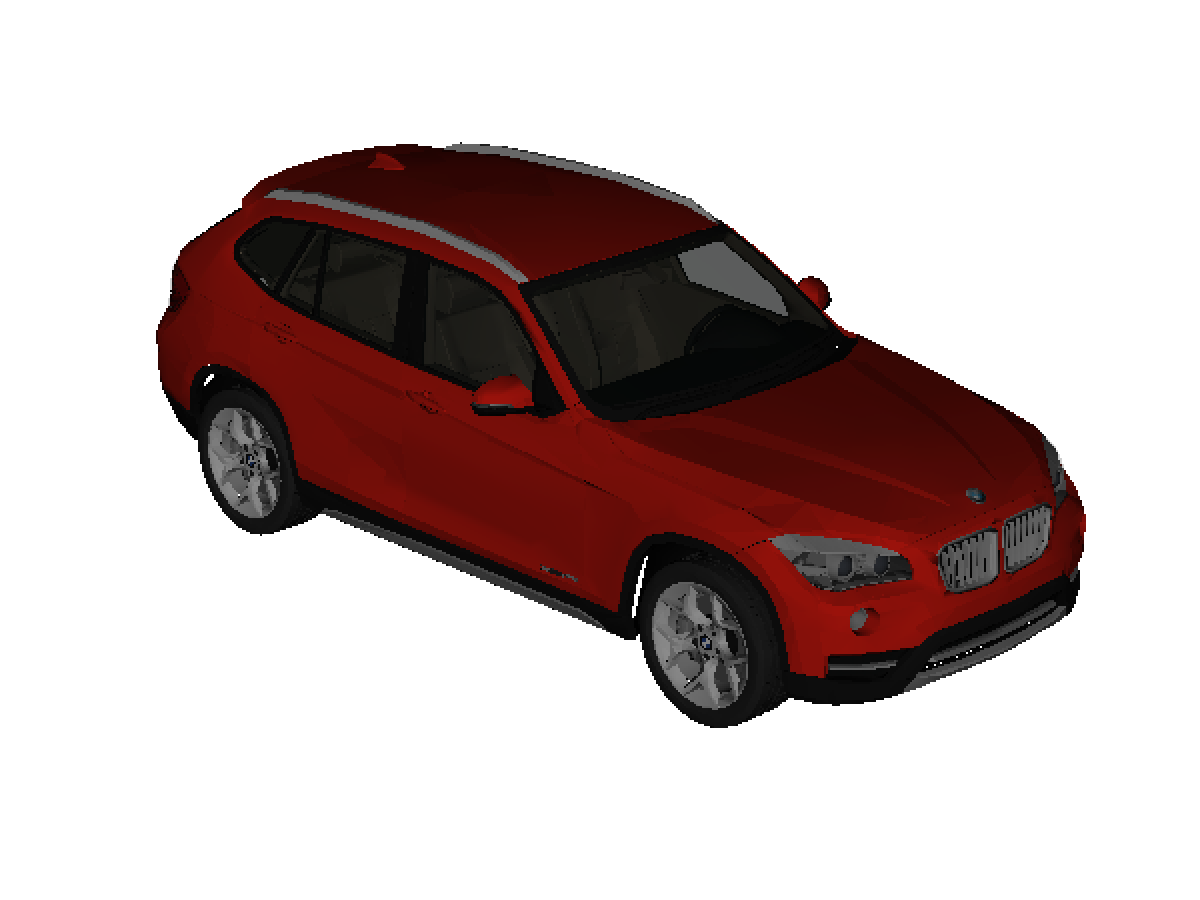
\includegraphics[width=0.16\linewidth]{rendering} &
              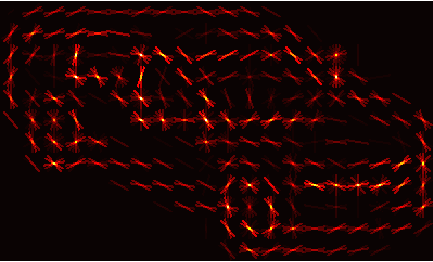
\includegraphics[width=0.18\linewidth]{whiten_all_crop} &
              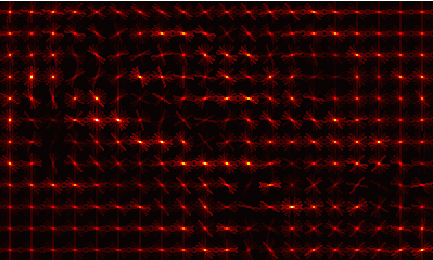
\includegraphics[width=0.18\linewidth]{whiten_all_neg_crop}  &
              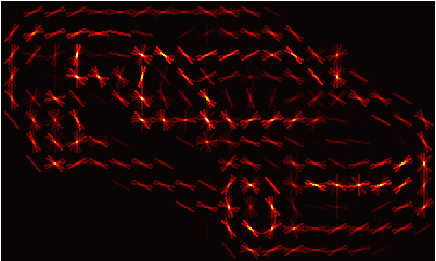
\includegraphics[width=0.18\linewidth]{whiten_non_zero_crop} &
              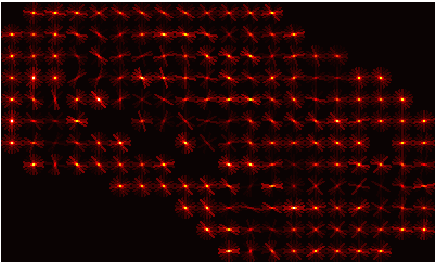
\includegraphics[width=0.18\linewidth]{whiten_non_zero_neg} \\
              \hline
            \end{tabular}
          \end{center}
        \end{figure}
      \end{block}

      %-- Block 2-2 --------------------------------------
      \begin{block}{Speedup using Conjugate Gradient method and FFT-Convolution}
        \begin{itemize}
          % \item Cholesky decomposition with Gaussian Elimination: $O(n^3)$
          \item Conjugate Gradient method time complexity: $O(n^2\kappa)$
          \item Cholesky Decomposition time complexity: $O(n^3)$
            % \begin{itemize}
            %   \item $\kappa$ condition number of the matrix $\Sigma$
            % \end{itemize}

          \begin{figure}[t]
            \begin{center}
            \begin{tabular}{ccc}
              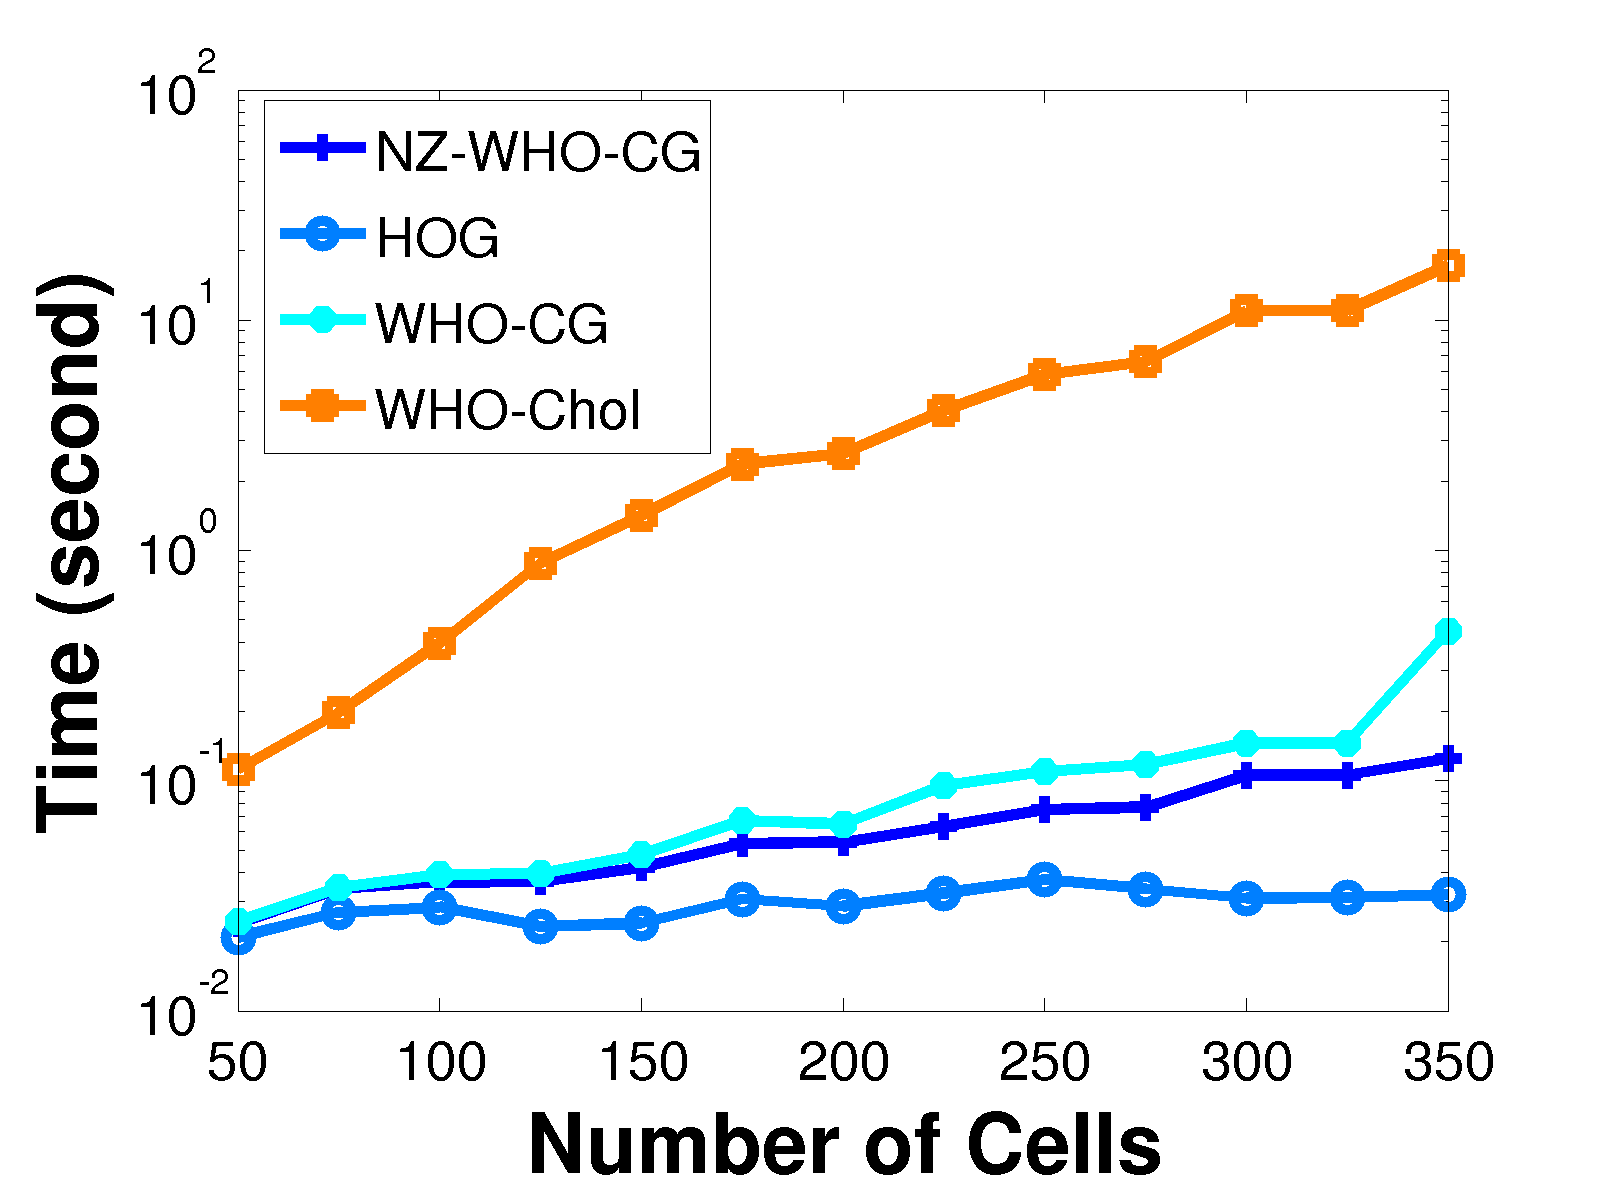
\includegraphics[width=0.3\linewidth]{whotime} &
              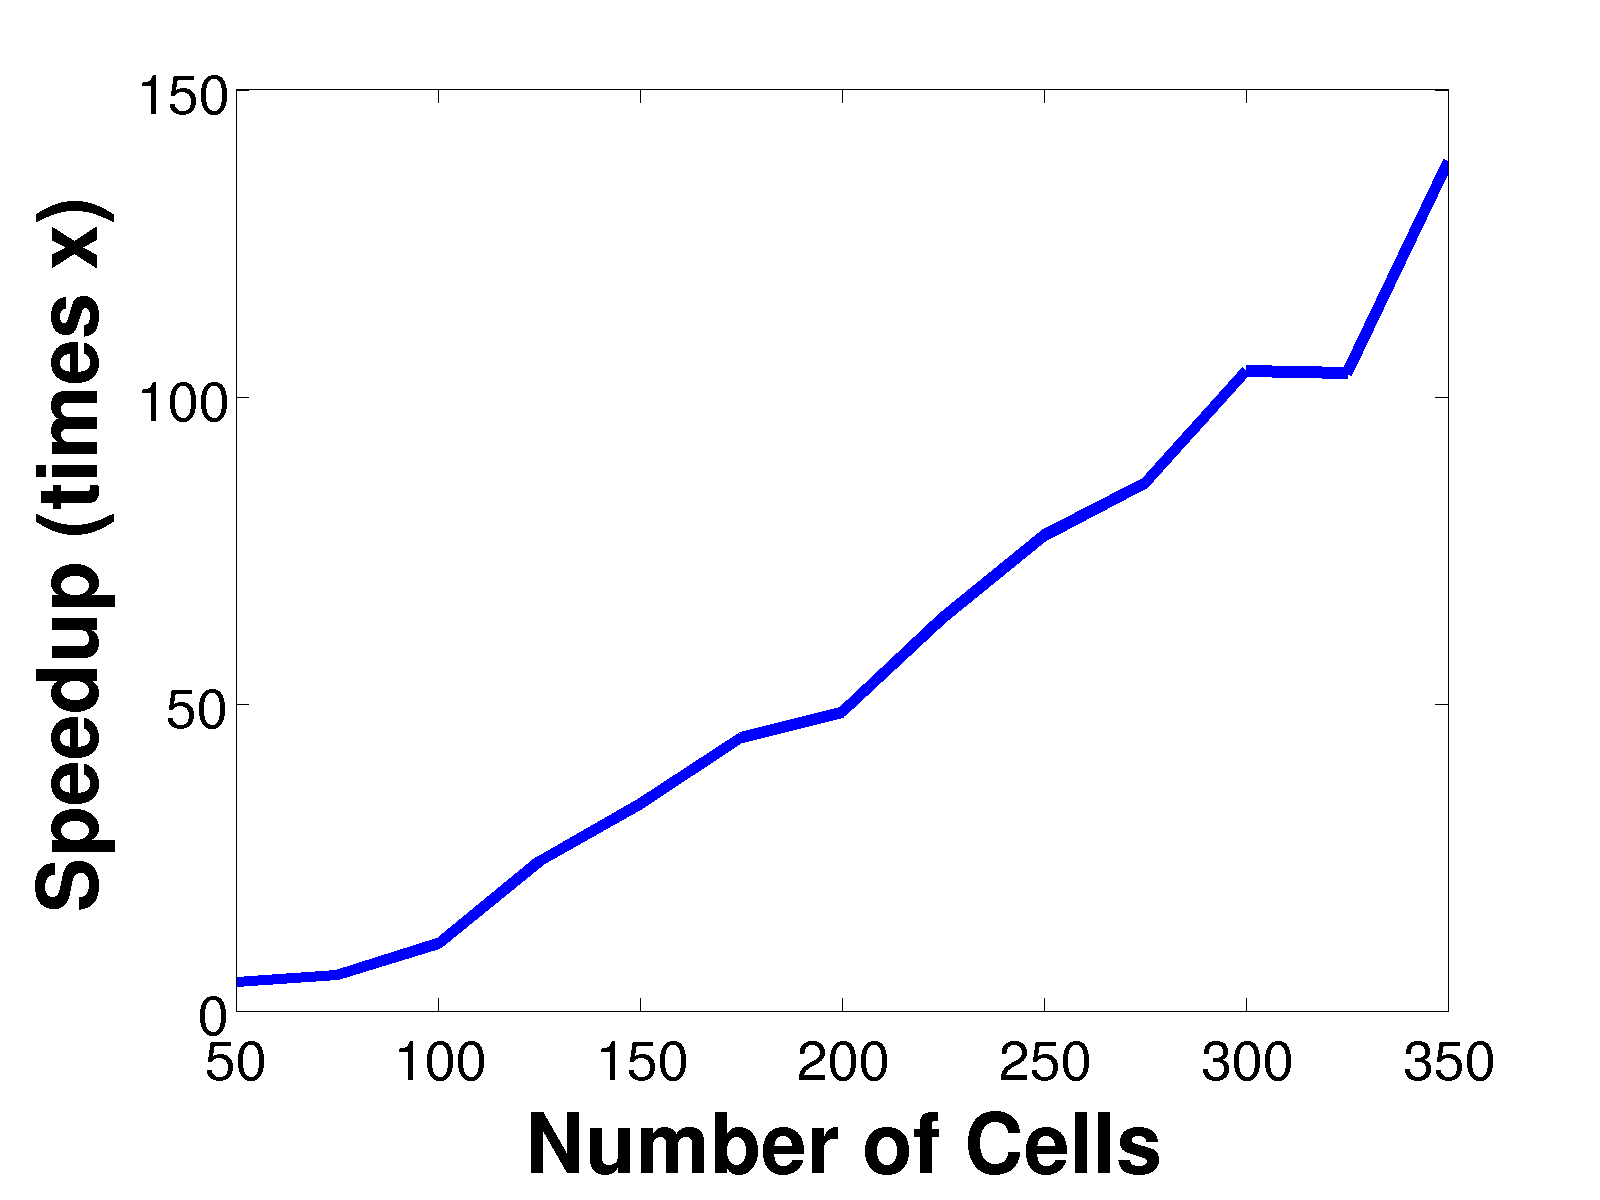
\includegraphics[width=0.3\linewidth]{speedup} &
              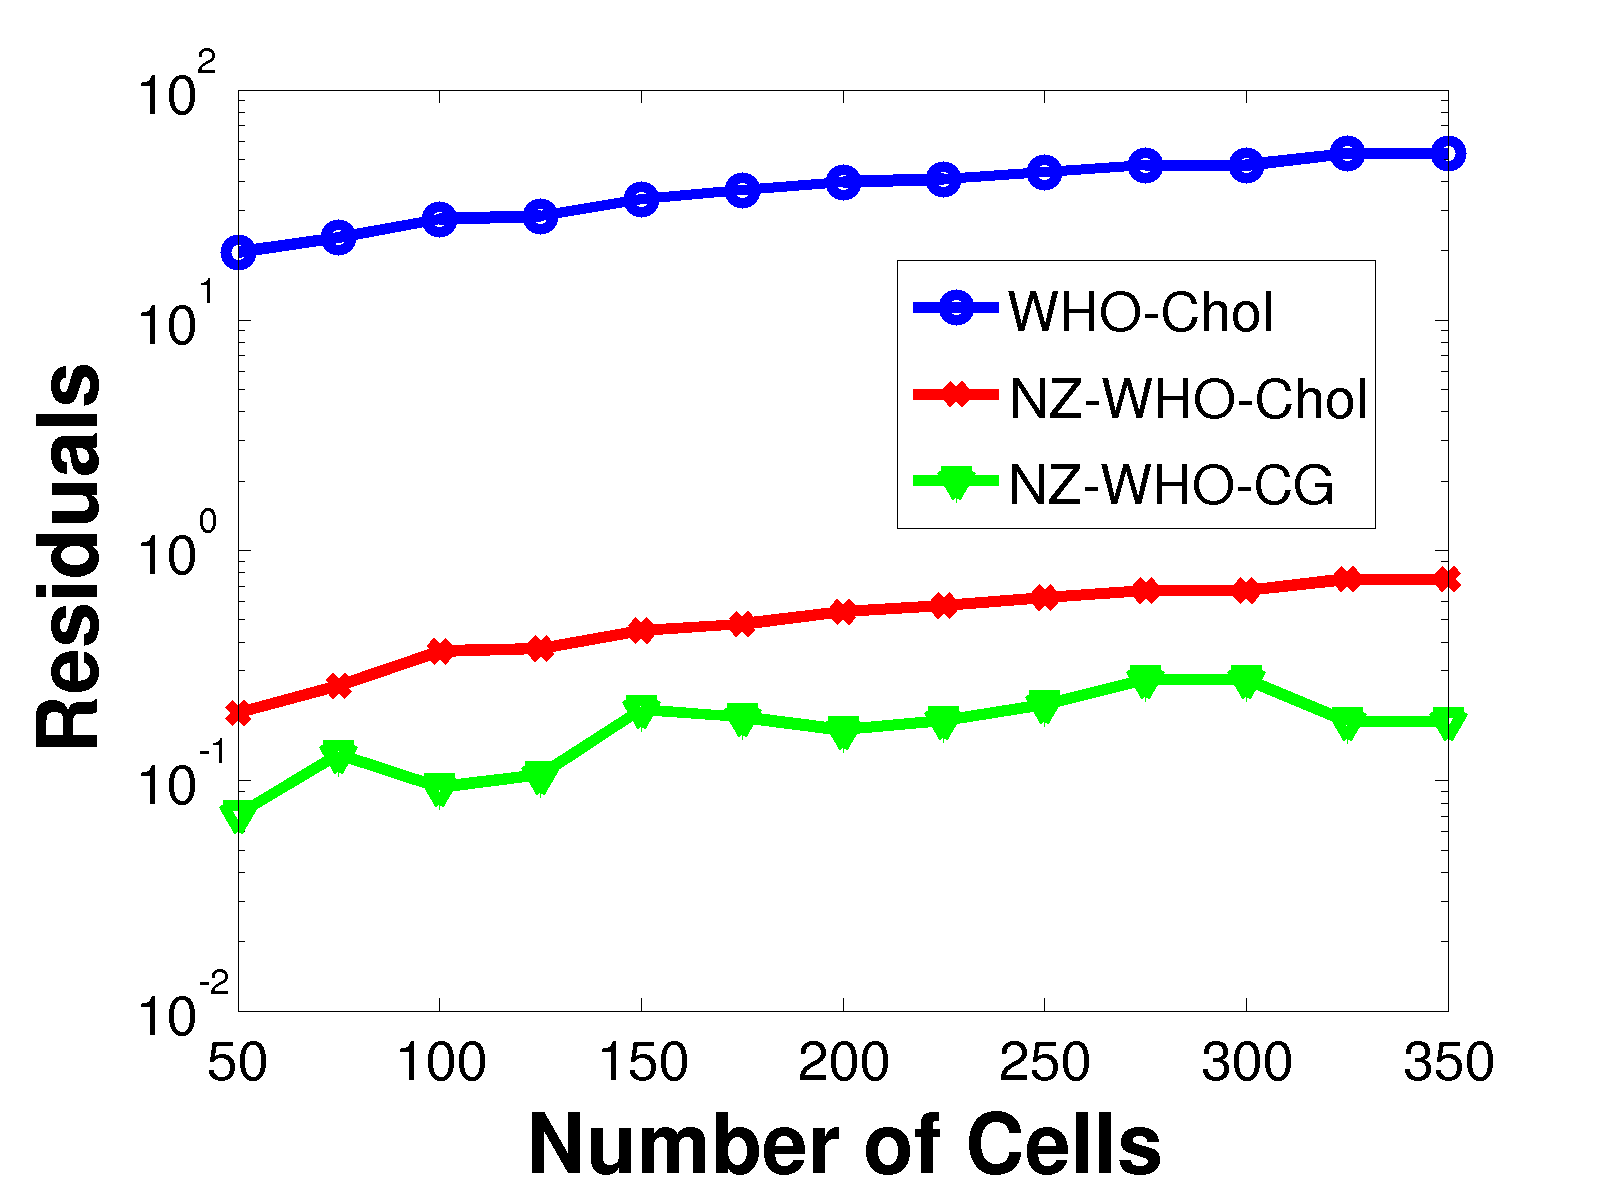
\includegraphics[width=0.3\linewidth]{residual} \\
           \end{tabular}
            \end{center}
            % \caption{(a) Runtime analysis of whitening. (b) final speedup
            %   of NZ-WHO vs. WHO. (c) Residuals of different method}
            % \label{fig:whotime}
          \end{figure}
          \item FFT-based Convolution
            % \begin{itemize}
            %   \item High resolution template $\sim 8,000$ dimensional features
            % \end{itemize}
        \end{itemize}
      \end{block}


    \end{column}%2



    %-----------------------------------------------------
    % Column 3
    %-----------------------------------------------------
    \begin{column}{0.23\linewidth}
      %-- Block 2-3 --------------------------------------
      \begin{block}{Experiments: NZ-WHO vs WHO}
        \begin{table}[!htbp]
          \small
          \setlength{\tabcolsep}{1pt}
          \centering
          \begin{tabular}{|c|c|r|c|r|}
            \hline
            Methods (AP/MPPE) & before calib.  & synth. time & after calib. & calib. time \\
            \hline\hline
            HOG      & 72.3 / 65.0          &  31ms  & 60.4 / 50.2           & 8.7 sec \\ 
            WHO  & 82.1 / \textbf{85.4} &  6162ms& 84.4 / 83.0           & 15.4 sec\\
            WHO-CG                 & 81.7 / 84.9          &  104ms & 83.7 / \textbf{87.3}  & 8.3 sec \\
            WHO-CG-Z               & 54.4 / 65.1          &  103ms & \textbf{92.8} / 86.7  & 8.7 sec \\
            NZ-WHO {\em (ours)} & \textbf{90.0} / 82.8 &   79ms & 90.3 / 86.8           & 8.5 sec \\
            \hline
          \end{tabular}
          % \caption{\small Average Precision (AP), Mean Precision in Pose Estimation
          %   (MPPE) of variants of WHO on 3D Object Classes cars, and their
          %   corresponding synthesis and calibration time per template.}
          \label{tab:who_initializations}
        \end{table}
      \end{block}



      %-- Block 3-2 --------------------------------------
      \begin{block}{Fine-Tuning via MCMC}
        \begin{itemize}
          \item Continuous parameter $\theta = [v, m, f]$
            % \begin{itemize}
            %   \item $v$ is the 3D rotation of the CAD model
            %   \item $m$ is the CAD model index
            %   \item $f$ is the focal length
            % \end{itemize}
            \begin{align}
                P(\theta| \mathcal{I}) & \sim e^{ \max_{s} w(\theta) \ast
                  \mathcal{T}_s(\mathcal{I})},
            \end{align}
            % \begin{itemize}
            %   \item $\max_{s} w(\theta) \ast T_s(\mathcal{I})$ is the maximum
            %     convolution score of NZ-WHO template with image features for
            %     all scale $s$
            % \end{itemize}
          \item Approximate the MAP solution
            \begin{itemize}
              \item using Single Component Metropolis-Hastings
            \end{itemize}
          % \item Proposal distributions for each component are
          %   \begin{align}
          %       g(\theta \rightarrow \theta(v_i^+)) & \sim
          %       \mathcal{N}(\theta_{v_i},\sigma_v) \quad \mbox{ for }\; i \in \{1,2,3\}\\
          %       g(\theta \rightarrow \theta(f^+)) & \sim \mathcal{N}(\theta_{f}, \sigma_f)\\
          %       g(\theta \rightarrow \theta(m^+)) & \sim (1-c) \delta(\theta_m) +
          %       c\,\textrm{Unif}(1,M)
          %   \end{align}
        \end{itemize}
      \end{block}


    \end{column}%3


    %-----------------------------------------------------
    % Column 4
    %-----------------------------------------------------       
    \begin{column}{0.23\linewidth}
      %-- Block 3-2
      \begin{block}{Conclusion}
        \begin{itemize}
          \item Non-Zero Whitened Histograms of Orientations (NZ-WHO)
            \begin{itemize}
              \item Generate E-LDA template from rendered 3D CAD data {\color{red} on-the-fly}
            \end{itemize}
          \item First attempt to simultaneously render and train exemplar detectors on-the-fly.
          \item Enrich the output of an existing object class detector
            \begin{itemize}
              \item 3D continuous pose and a 3D CAD model exemplar.
            \end{itemize}
        \end{itemize}
      \end{block}

      % \begin{block}{Acknowledgement}
      %   \small
      %   We acknowledge the support of NSF CAREER grant (N1054127),
      %   Ford-Stanford Innovation Alliance Award, DARPA, Korea Foundation for
      %   Advanced Studies, Fulbright New Zealand and the Max Planck Center for
      %   Visual Computing \& Communication.
      % \end{block}

      % \begin{block}{References}
      %   {\footnotesize
      %   \bibliographystyle{../ieee}
      %   \bibliography{2349_poster}
      %   }
      % \end{block}
    \end{column}%4
  \end{columns}





  %---------------------------------------------------------
  % New Row
  %---------------------------------------------------------
  \vspace{0.1em}
  \begin{columns}[t]
    \begin{column}{0.3\linewidth}
      %-- Block 1-3 --------------------------------------
      \begin{block}{Overview}
        % Figure
        \begin{figure}[t]
          \centering
          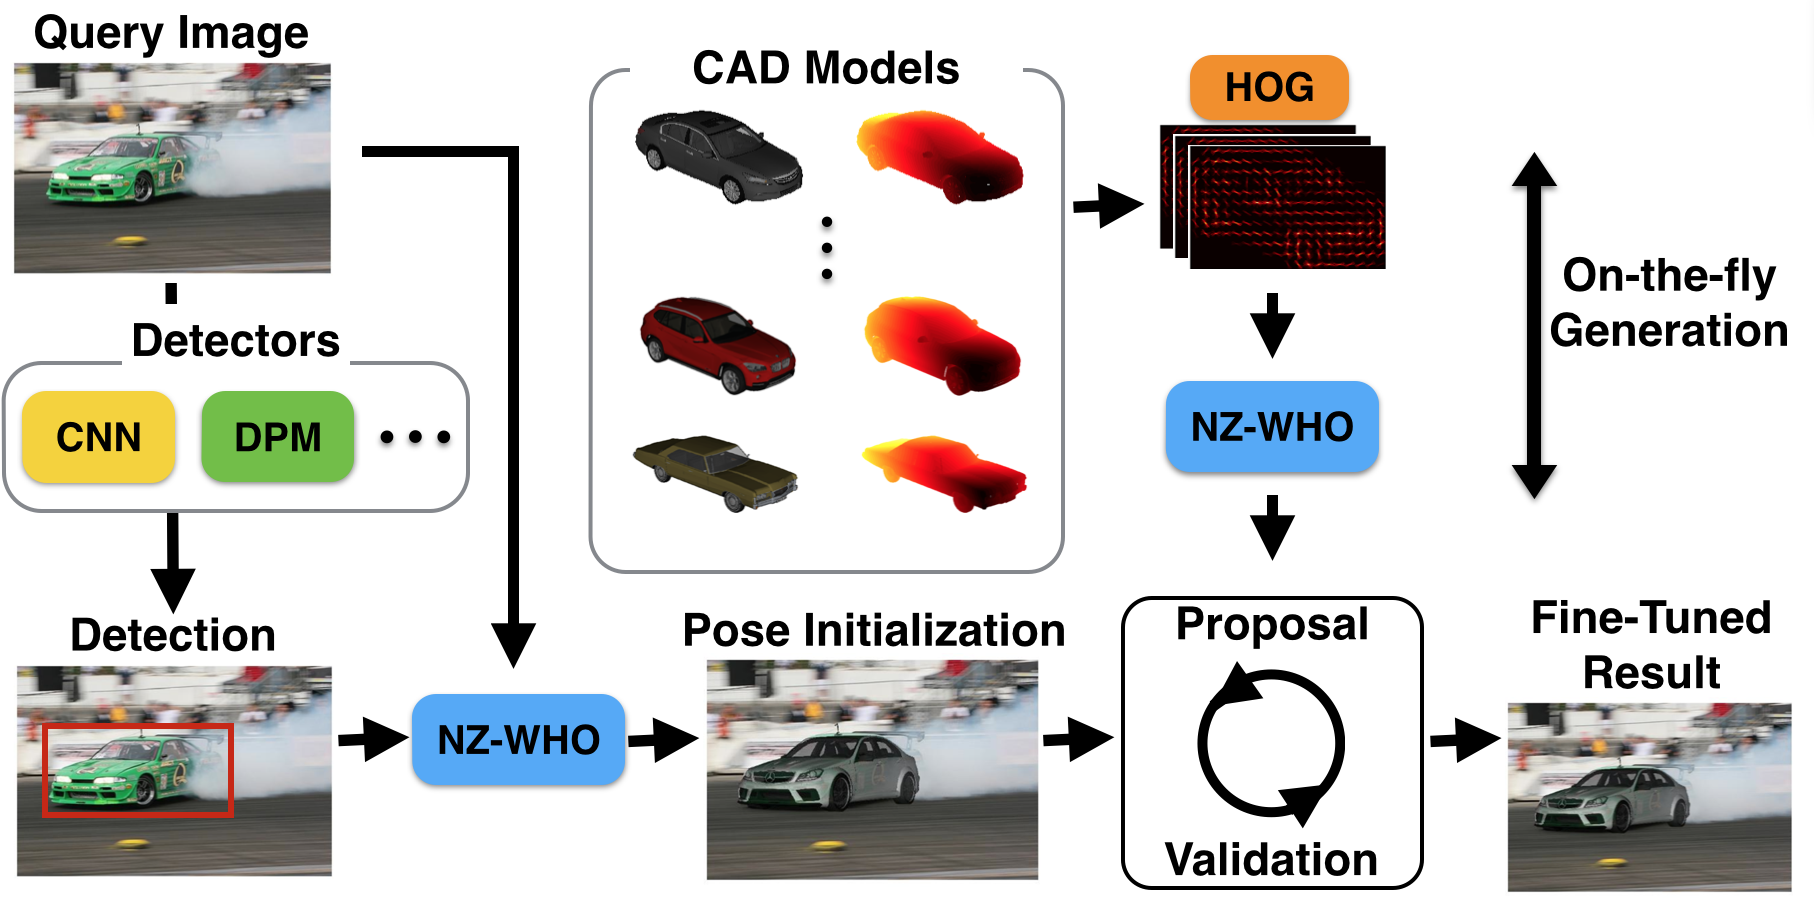
\includegraphics[width=0.95\linewidth]{front} % \\[-5pt]
        \end{figure}
        % \vspace{-1.0em}

        % \begin{itemize}
        %   \item Create an ensemble of NZ-WHO templates
        %   \item Initialize viewpoint
        %   \item Propose and validate using Single component Metropolis-Hastings
        %     algorithm
        % \end{itemize}
      \end{block}
    \end{column}

    \begin{column}{0.3\linewidth}

      %-- Block 3-3 --------------------------------------
      \begin{block}{Experiments: OBJECT 3D}
        \begin{figure}
          \begin{center}
          \setlength\tabcolsep{0pt}
          \begin{tabular}{c|c}
            \hline
            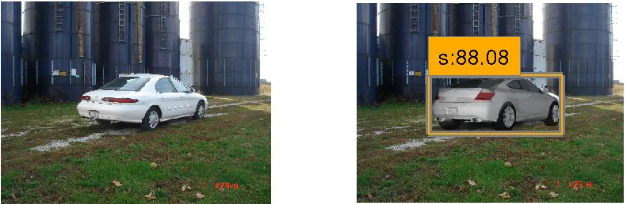
\includegraphics[width=0.40\linewidth]{supp/car32.png} &
            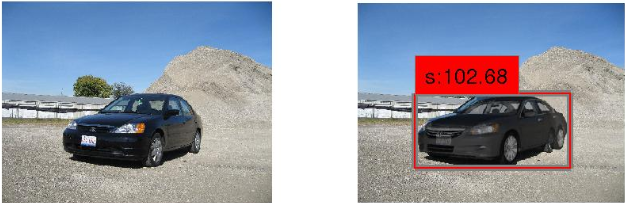
\includegraphics[width=0.40\linewidth]{supp/car26.png} \\
            % 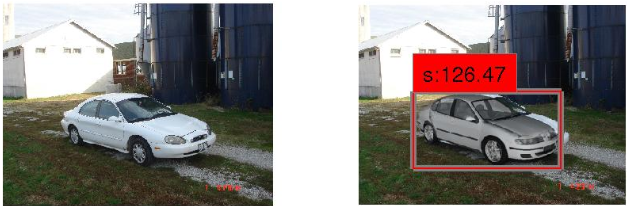
\includegraphics[width=0.40\linewidth]{supp/car20.png} & 
            % 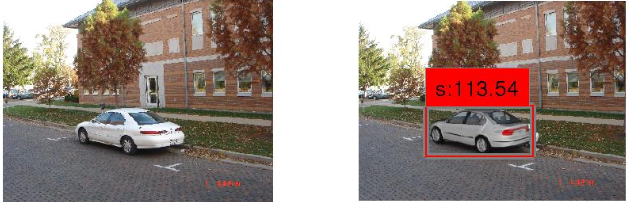
\includegraphics[width=0.40\linewidth]{supp/car31.png} \\
            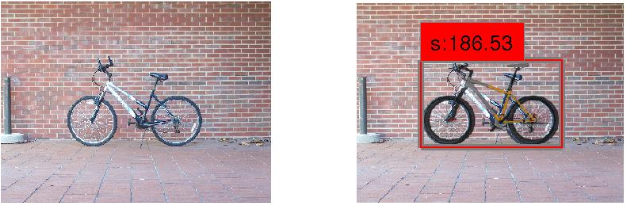
\includegraphics[width=0.40\linewidth]{supp/bicycle16.png} &
            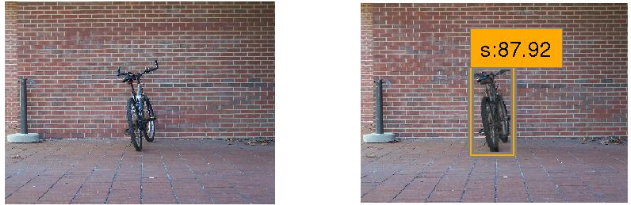
\includegraphics[width=0.40\linewidth]{supp/bicycle12.png} \\
            % 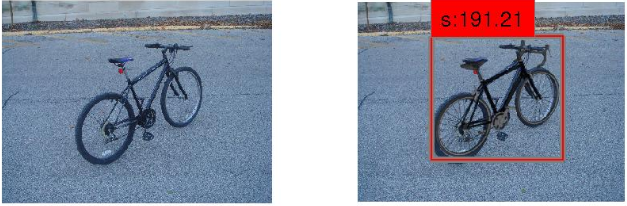
\includegraphics[width=0.40\linewidth]{supp/bicycle15.png} &
            % 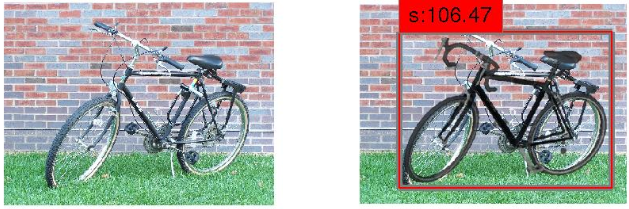
\includegraphics[width=0.40\linewidth]{supp/bicycle10.png} \\
            \hline
          %  (c) & (d) \\[0pt]
          \end{tabular}
          \end{center}
          % \caption{\small Detection results on 3D Object Classes. Original image
          %   (left) and detection result overlaid on top (right).}
          % \label{fig:3dobject_vis}
        \end{figure}

        \begin{table}[!htbp]
          \begin{center}
            \begin{tabular}{|c|c|c|c|}
            \hline
            AP/MPPE& Ours & ALM & DPM-VOC+VP \\
            \hline\hline
            car     & \textbf{99.8} / 91.7 & 98.4 / 93.4 & \textbf{99.8} / \textbf{97.5} \\ 
            bicycle & 93.0 / 90.9          & 93.0 / 91.4 & \textbf{98.8} / \textbf{97.5} \\
            \hline
            \end{tabular}
          \end{center}
          % \caption{Average Precision (AP) and Mean Precision in Pose
          %   Estimation (MPPE) on 3D Object Classes~\cite{Savarese07} cars.}% Our method produces high quality 2D-3D matching yet performs on par with state-of-the art detectors.}
          % \label{tab:3dobject}
        \end{table}


      \end{block}
    \end{column}

    \begin{column}{0.39\linewidth}
      %-- Block 3-1
      \begin{block}{Experiments: PASCAL3D}
        \begin{figure}
        \setlength\tabcolsep{1pt}
        \centering
        \begin{tabular}{|c|c|c|c|c|}
          \hline
          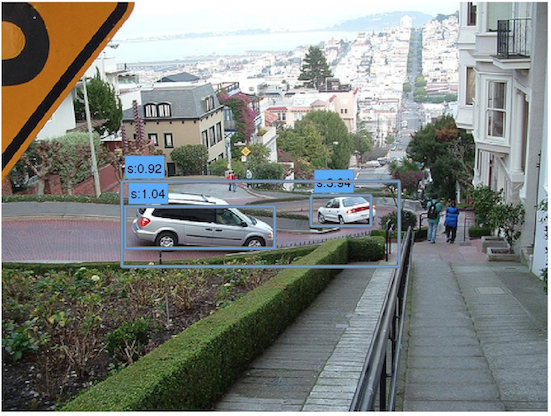
\includegraphics[width=0.24\textwidth]{car_cnn/1a.png} &   
          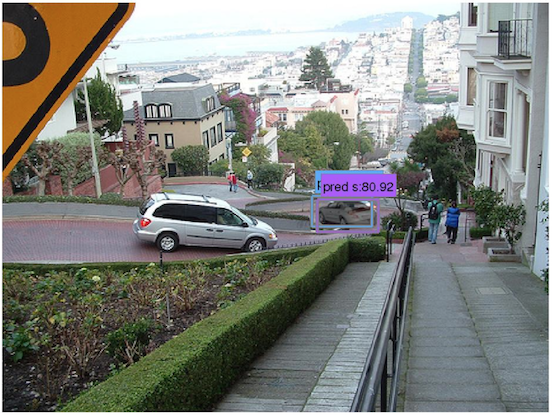
\includegraphics[width=0.24\textwidth]{car_cnn/1b.png} &   
          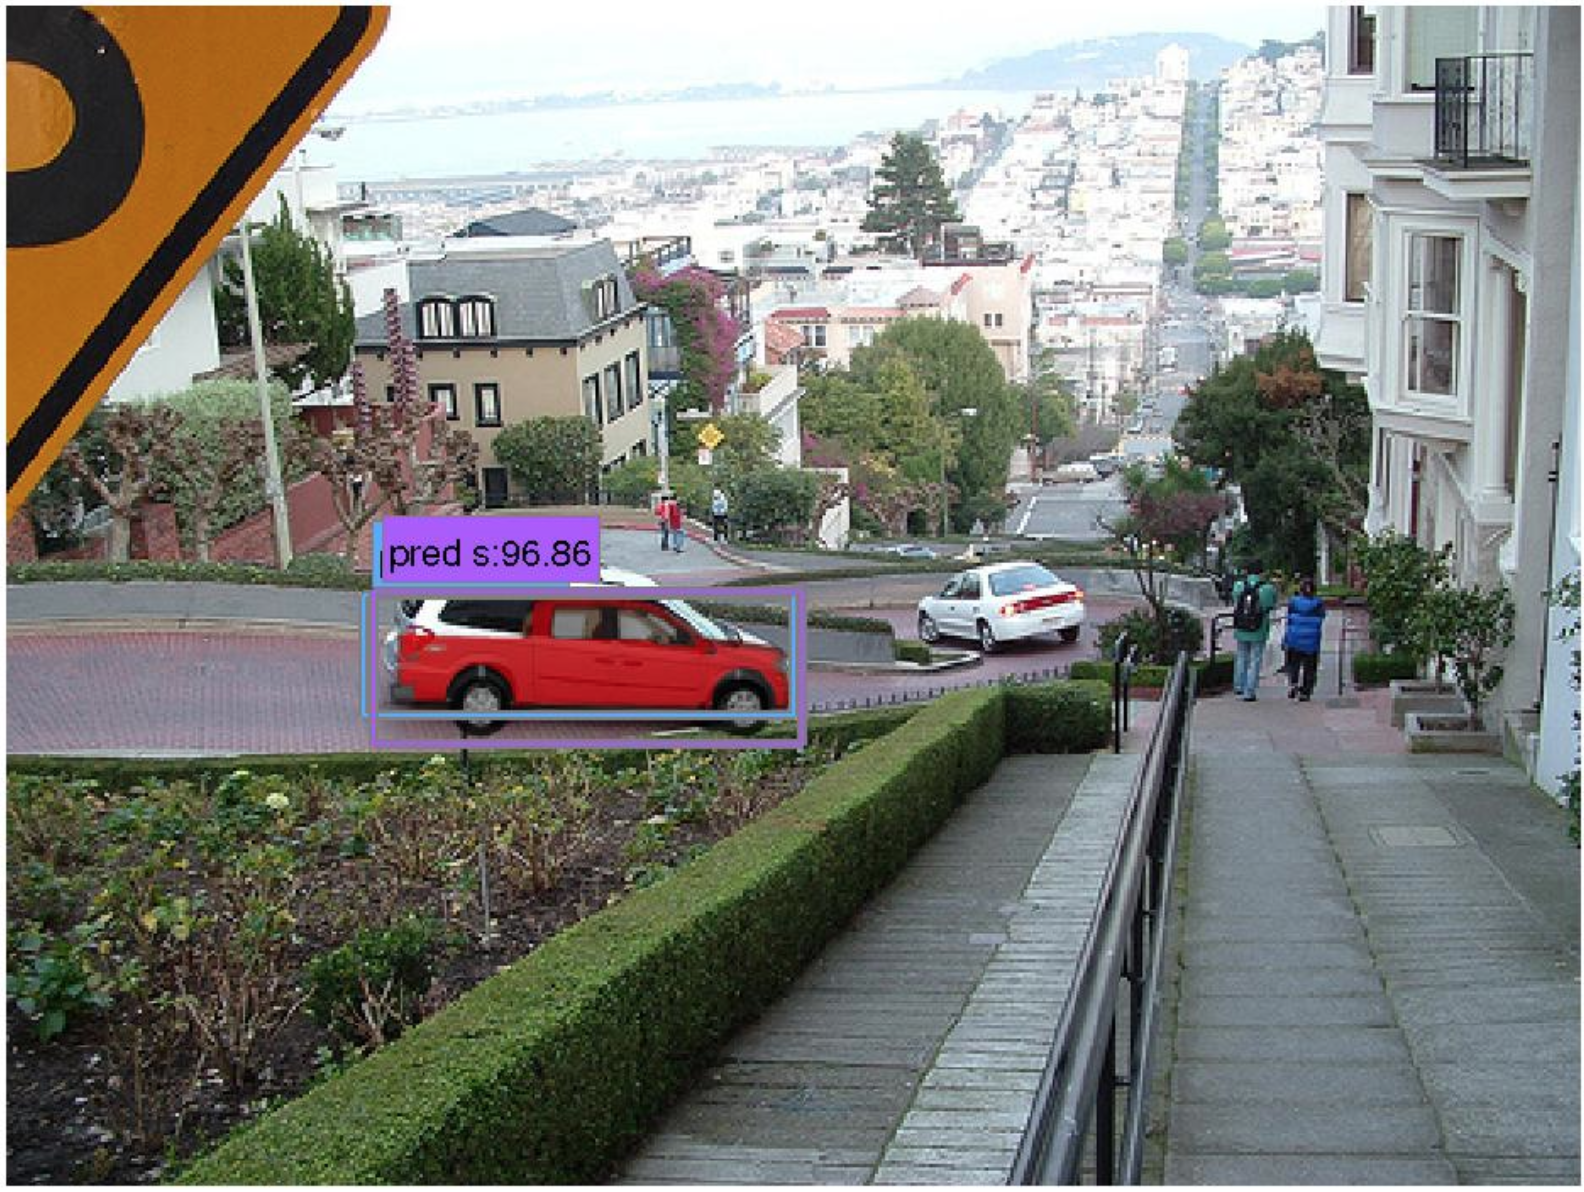
\includegraphics[width=0.24\textwidth]{car_cnn/1c.png} &   
          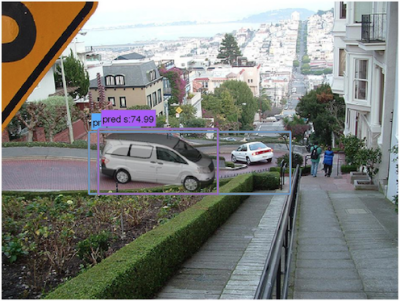
\includegraphics[width=0.24\textwidth]{car_cnn/1d.png}  \\  
          \hline
          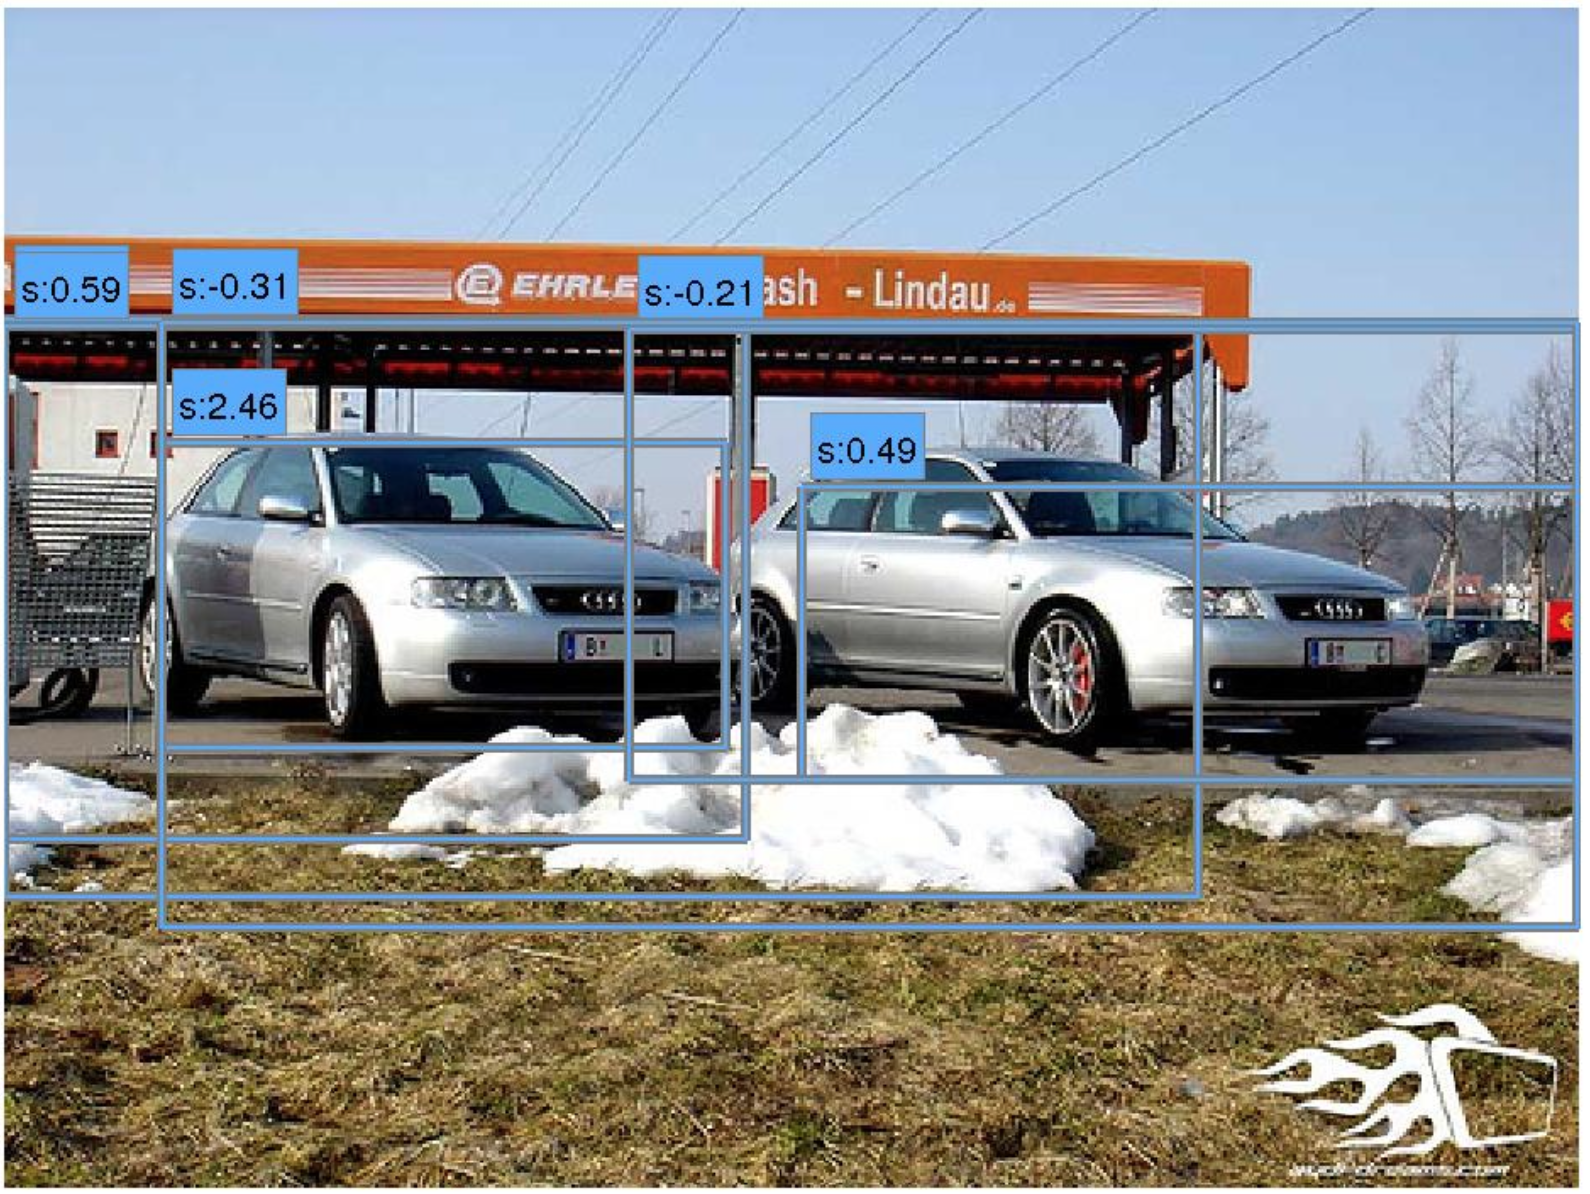
\includegraphics[width=0.24\textwidth]{car_cnn/2a.png} &   
          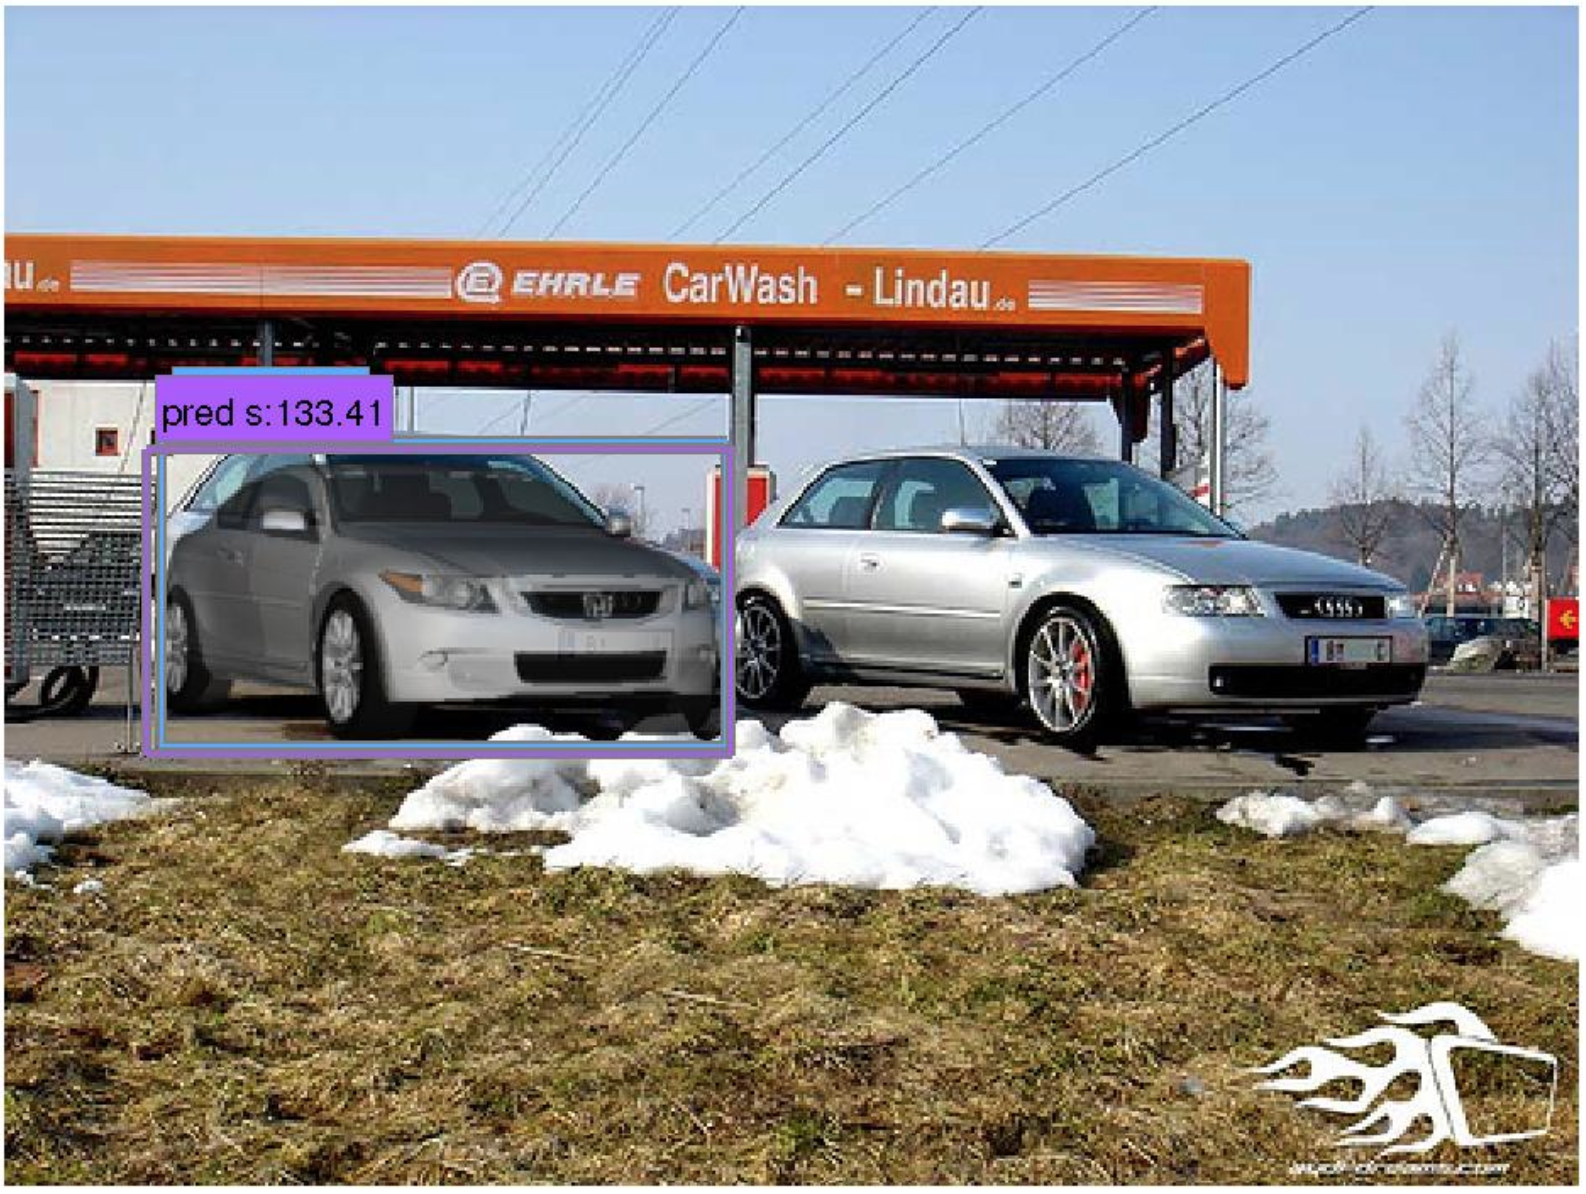
\includegraphics[width=0.24\textwidth]{car_cnn/2b.png} &   
          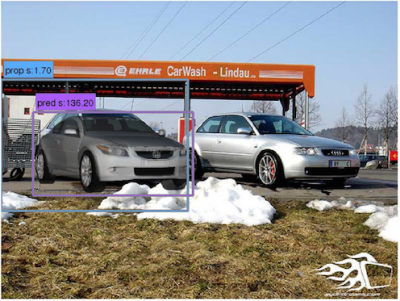
\includegraphics[width=0.24\textwidth]{car_cnn/2c.png} &   
          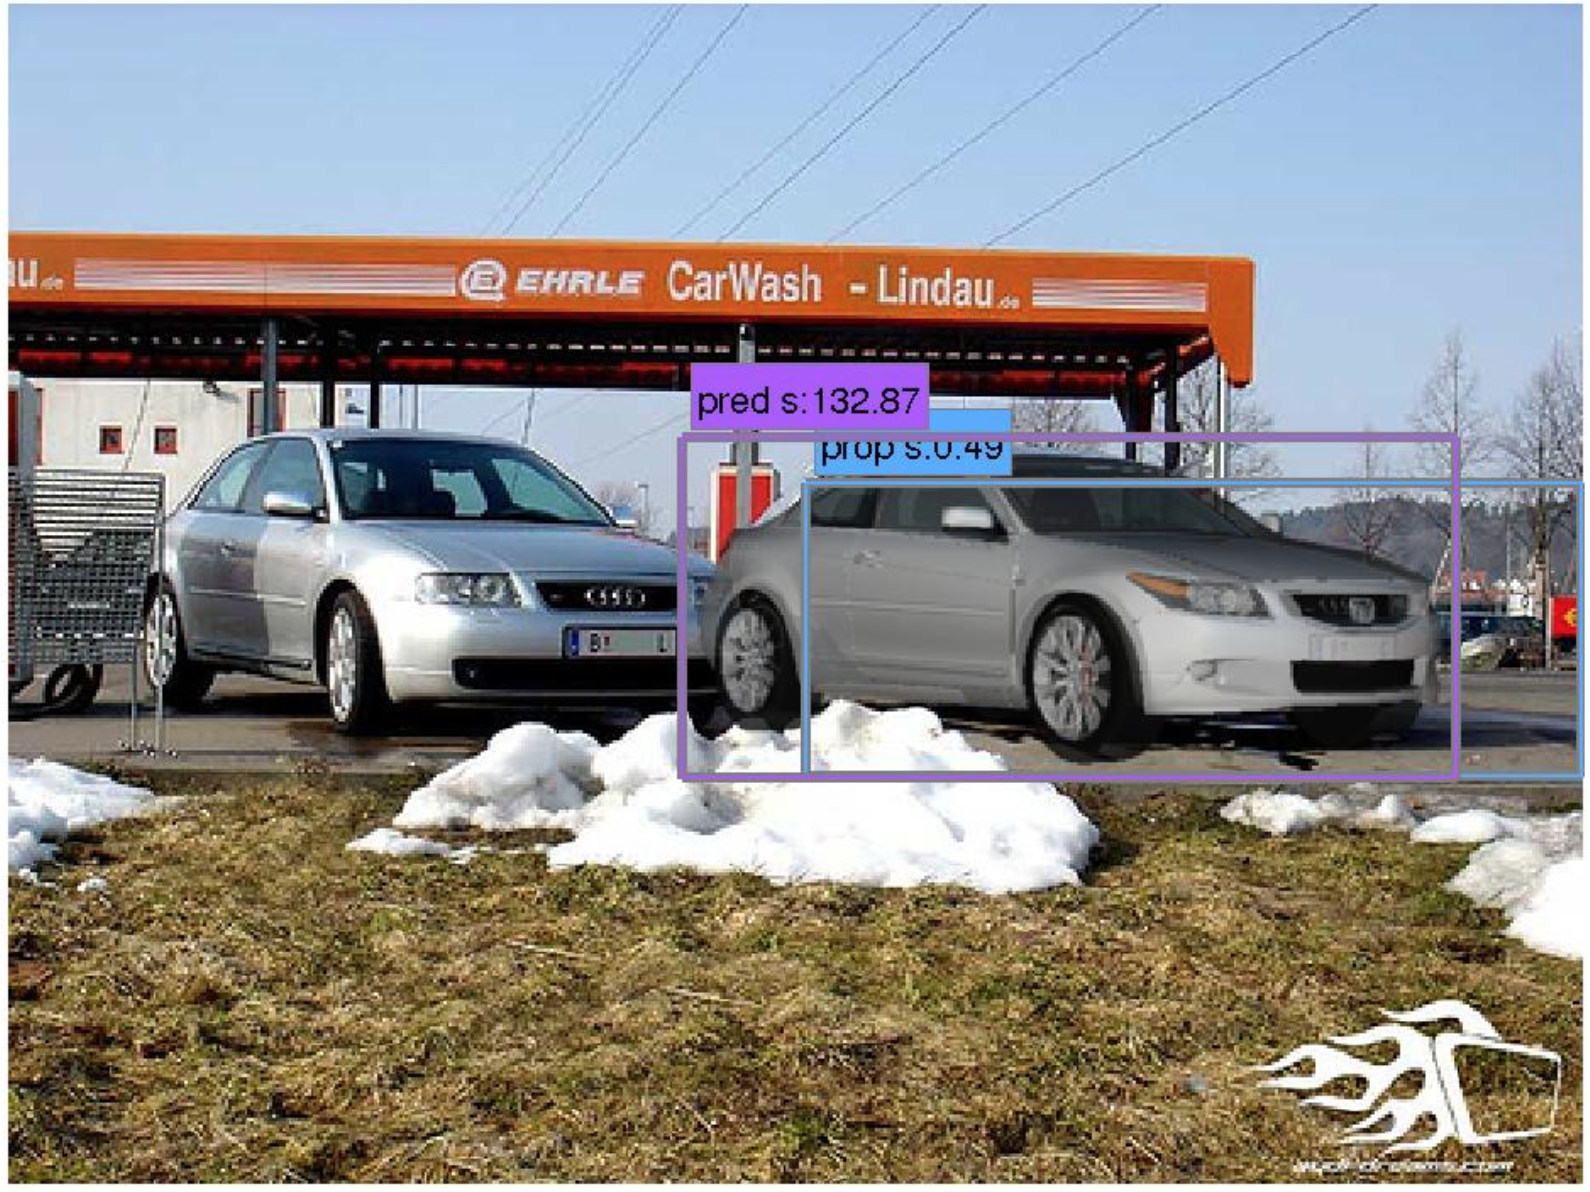
\includegraphics[width=0.24\textwidth]{car_cnn/2e.png}  \\  
          \hline
          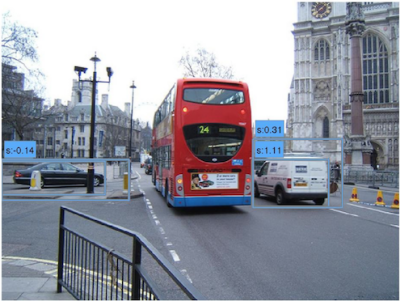
\includegraphics[width=0.24\textwidth]{car_cnn/4a.png} &   
          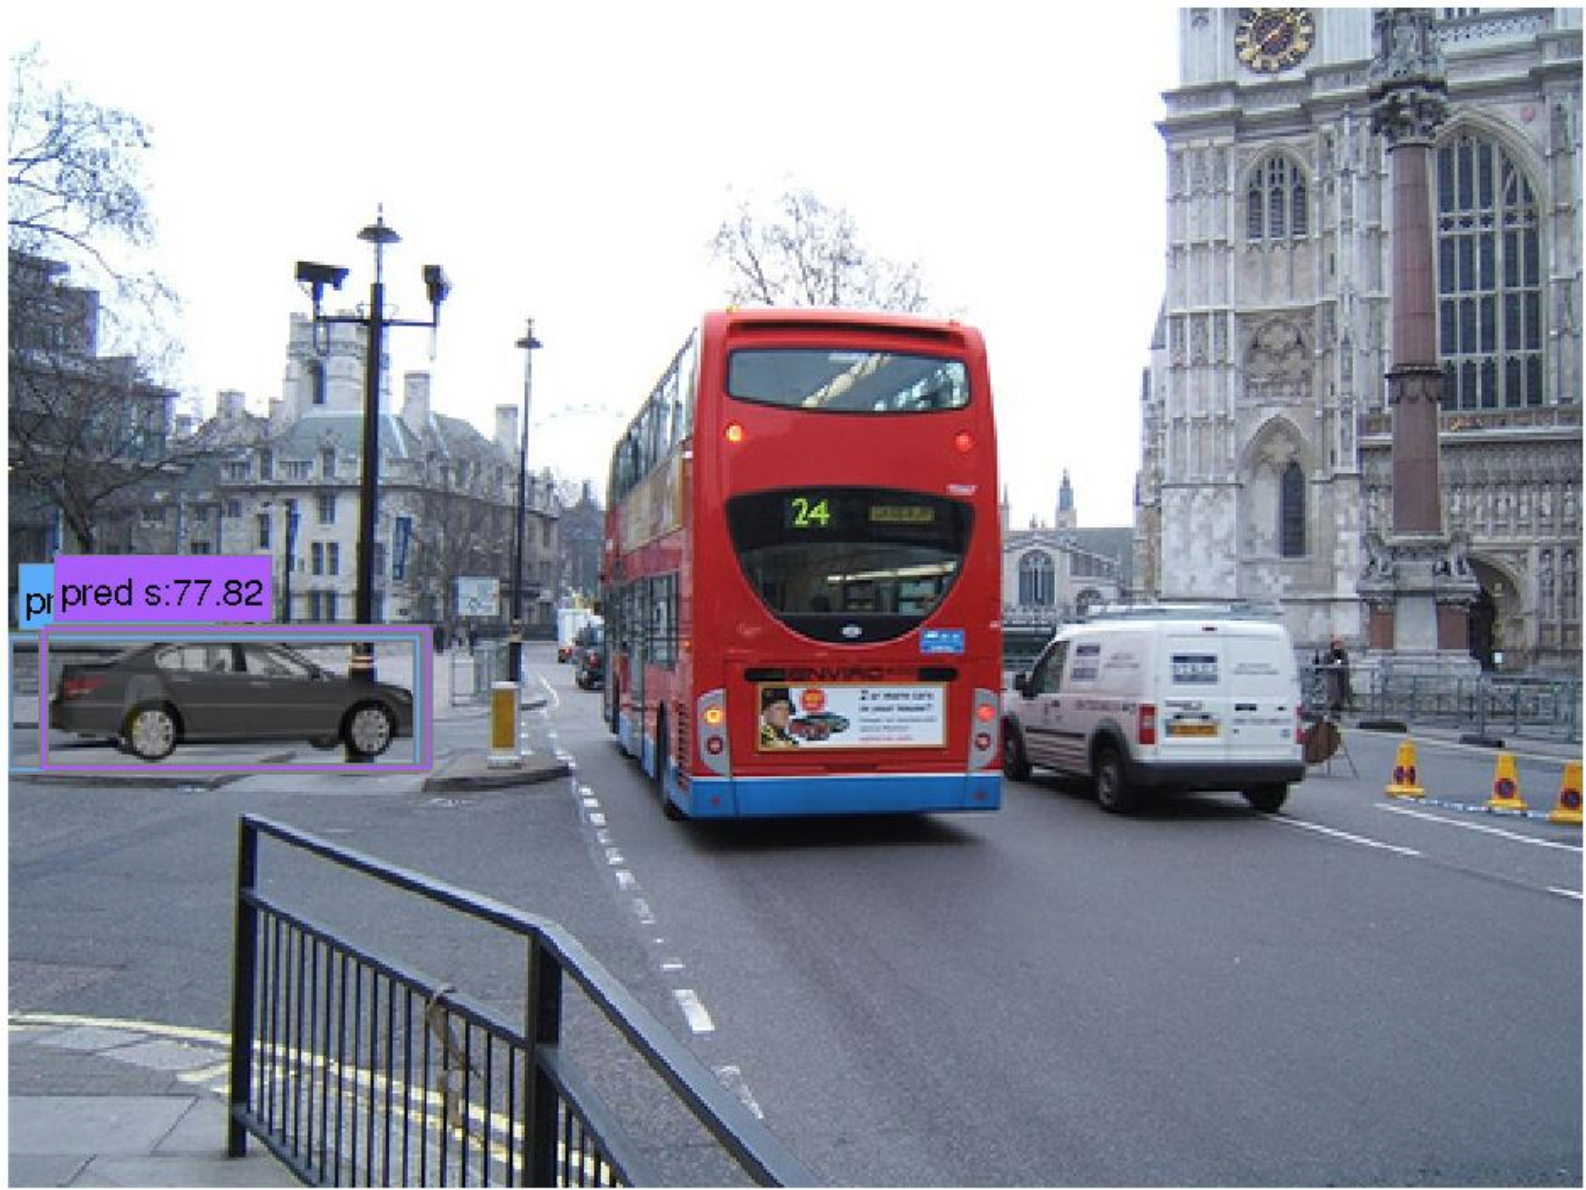
\includegraphics[width=0.24\textwidth]{car_cnn/4b.png} &   
          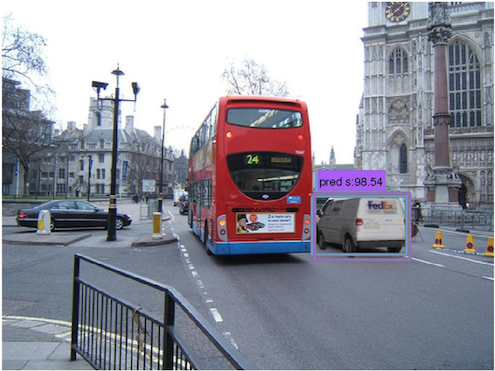
\includegraphics[width=0.24\textwidth]{car_cnn/4c.png} &   
          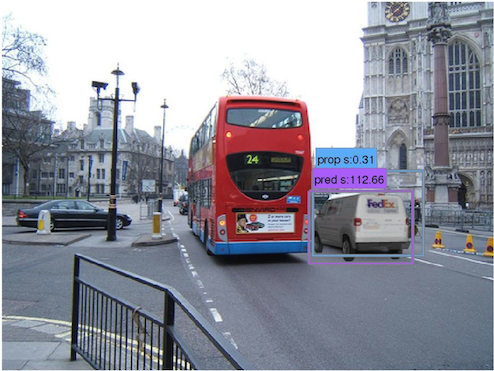
\includegraphics[width=0.24\textwidth]{car_cnn/4d.png}  \\  
        %    \hline
        %   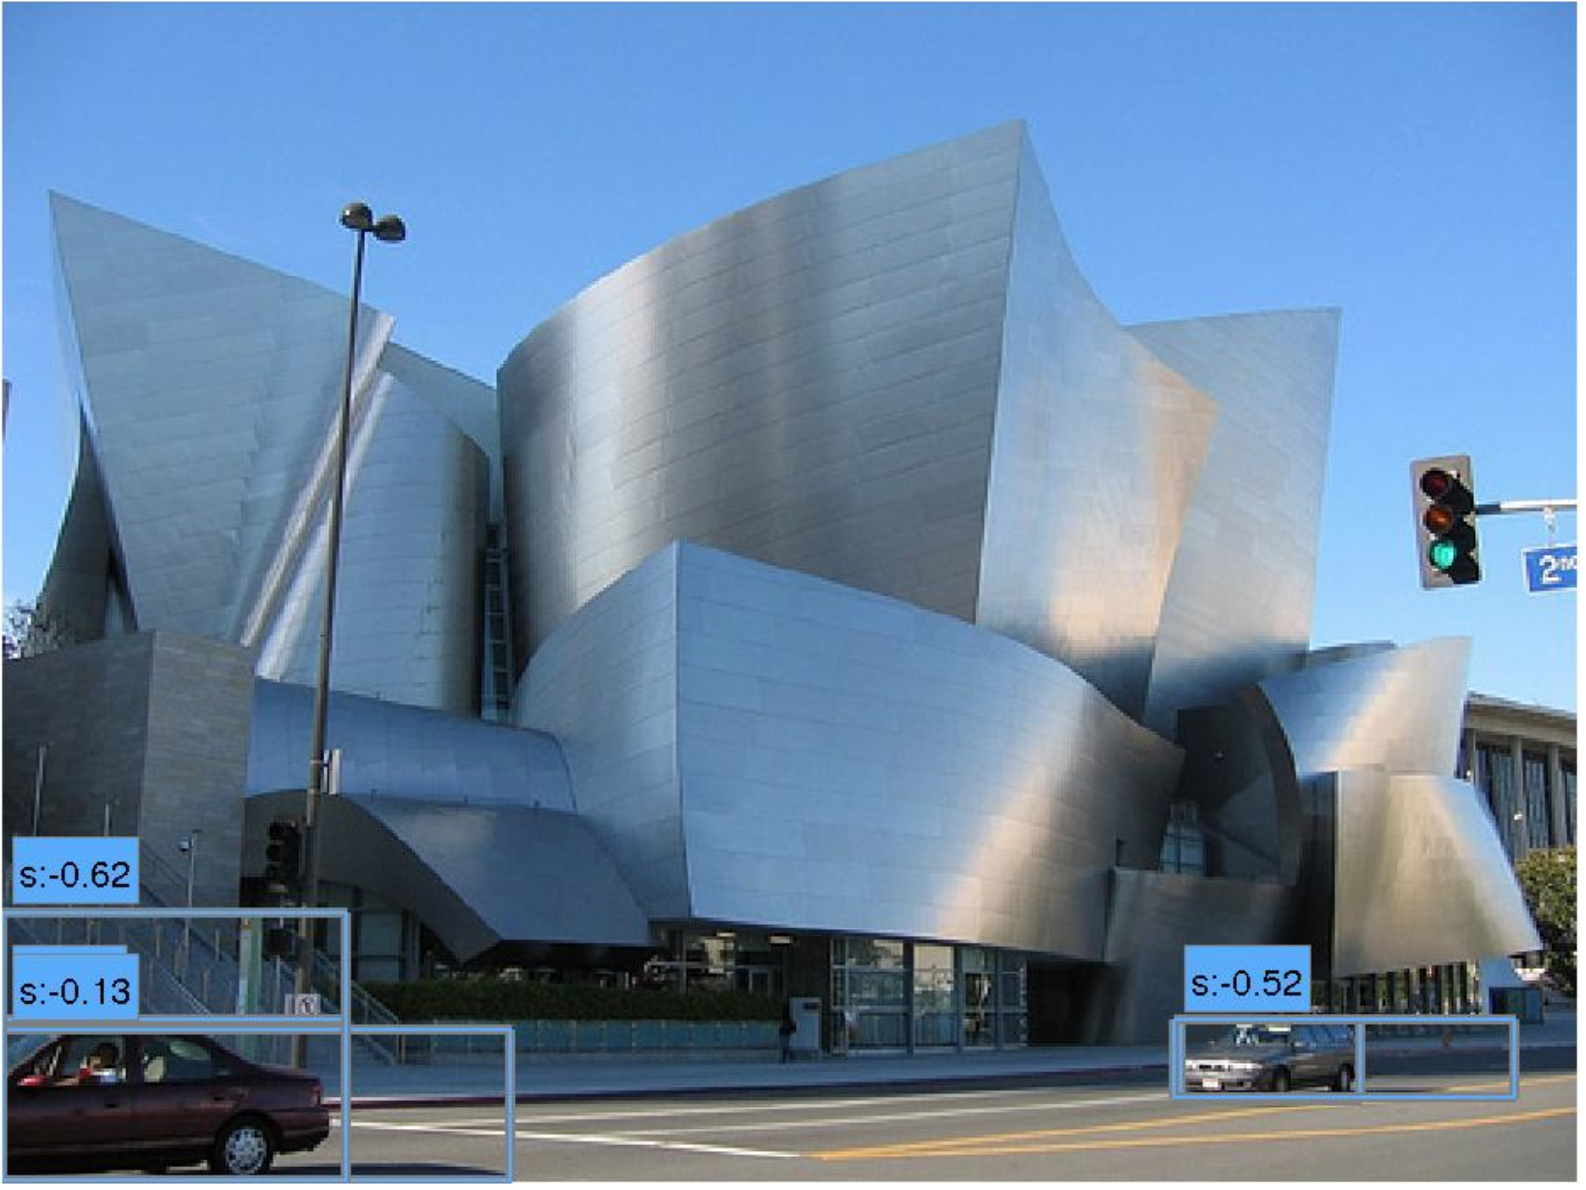
\includegraphics[width=0.24\textwidth]{car_cnn/10a.png} &   
        %   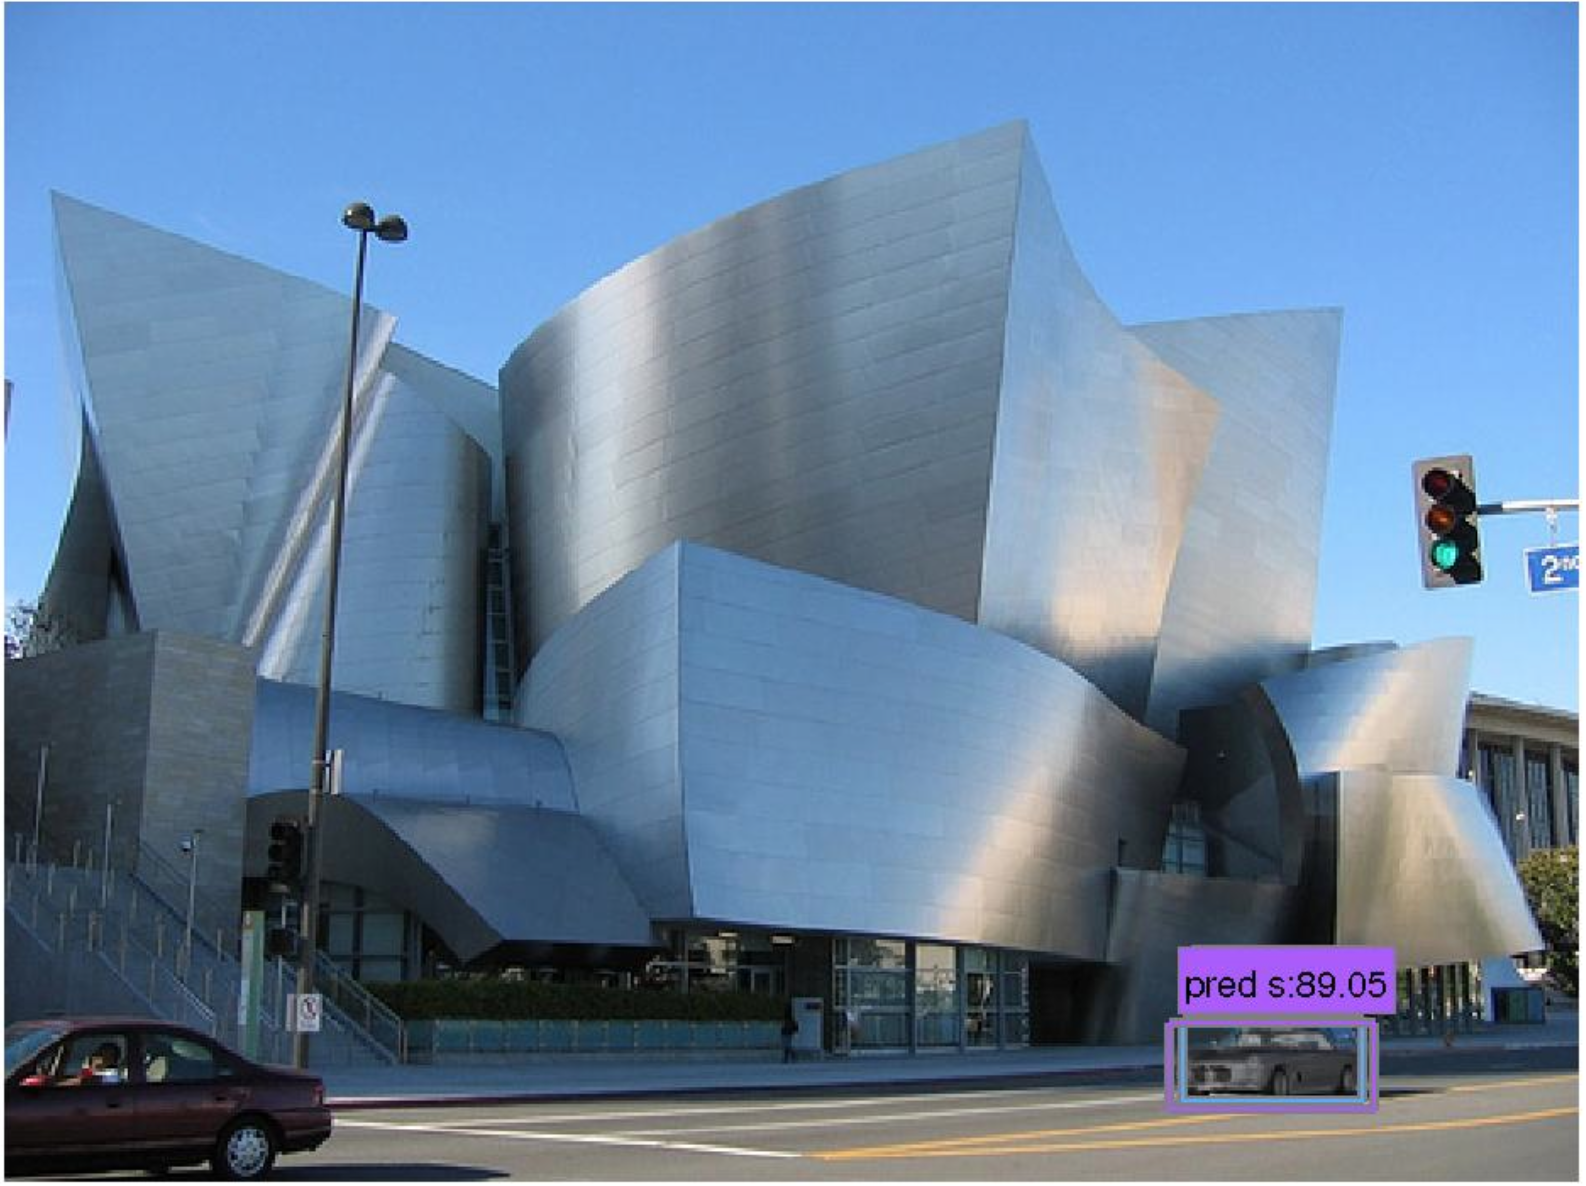
\includegraphics[width=0.24\textwidth]{car_cnn/10b.png} &   
        %   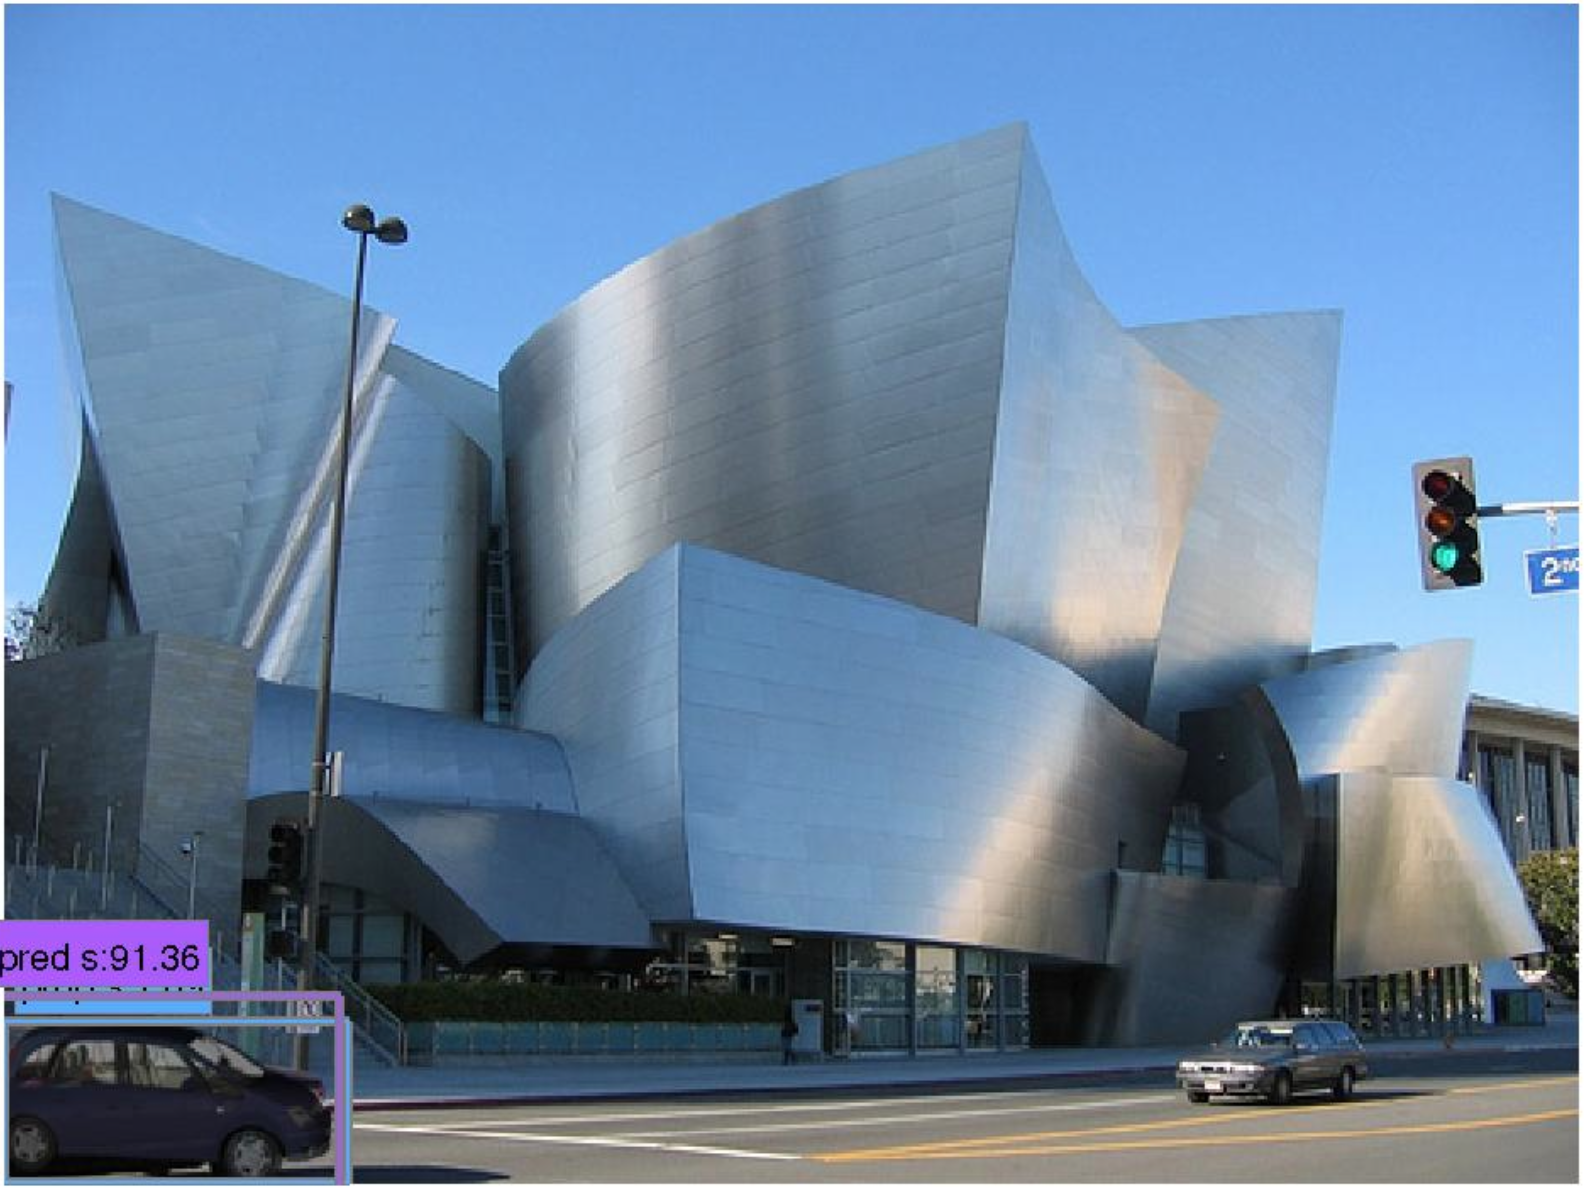
\includegraphics[width=0.24\textwidth]{car_cnn/10c.png} &   
        %   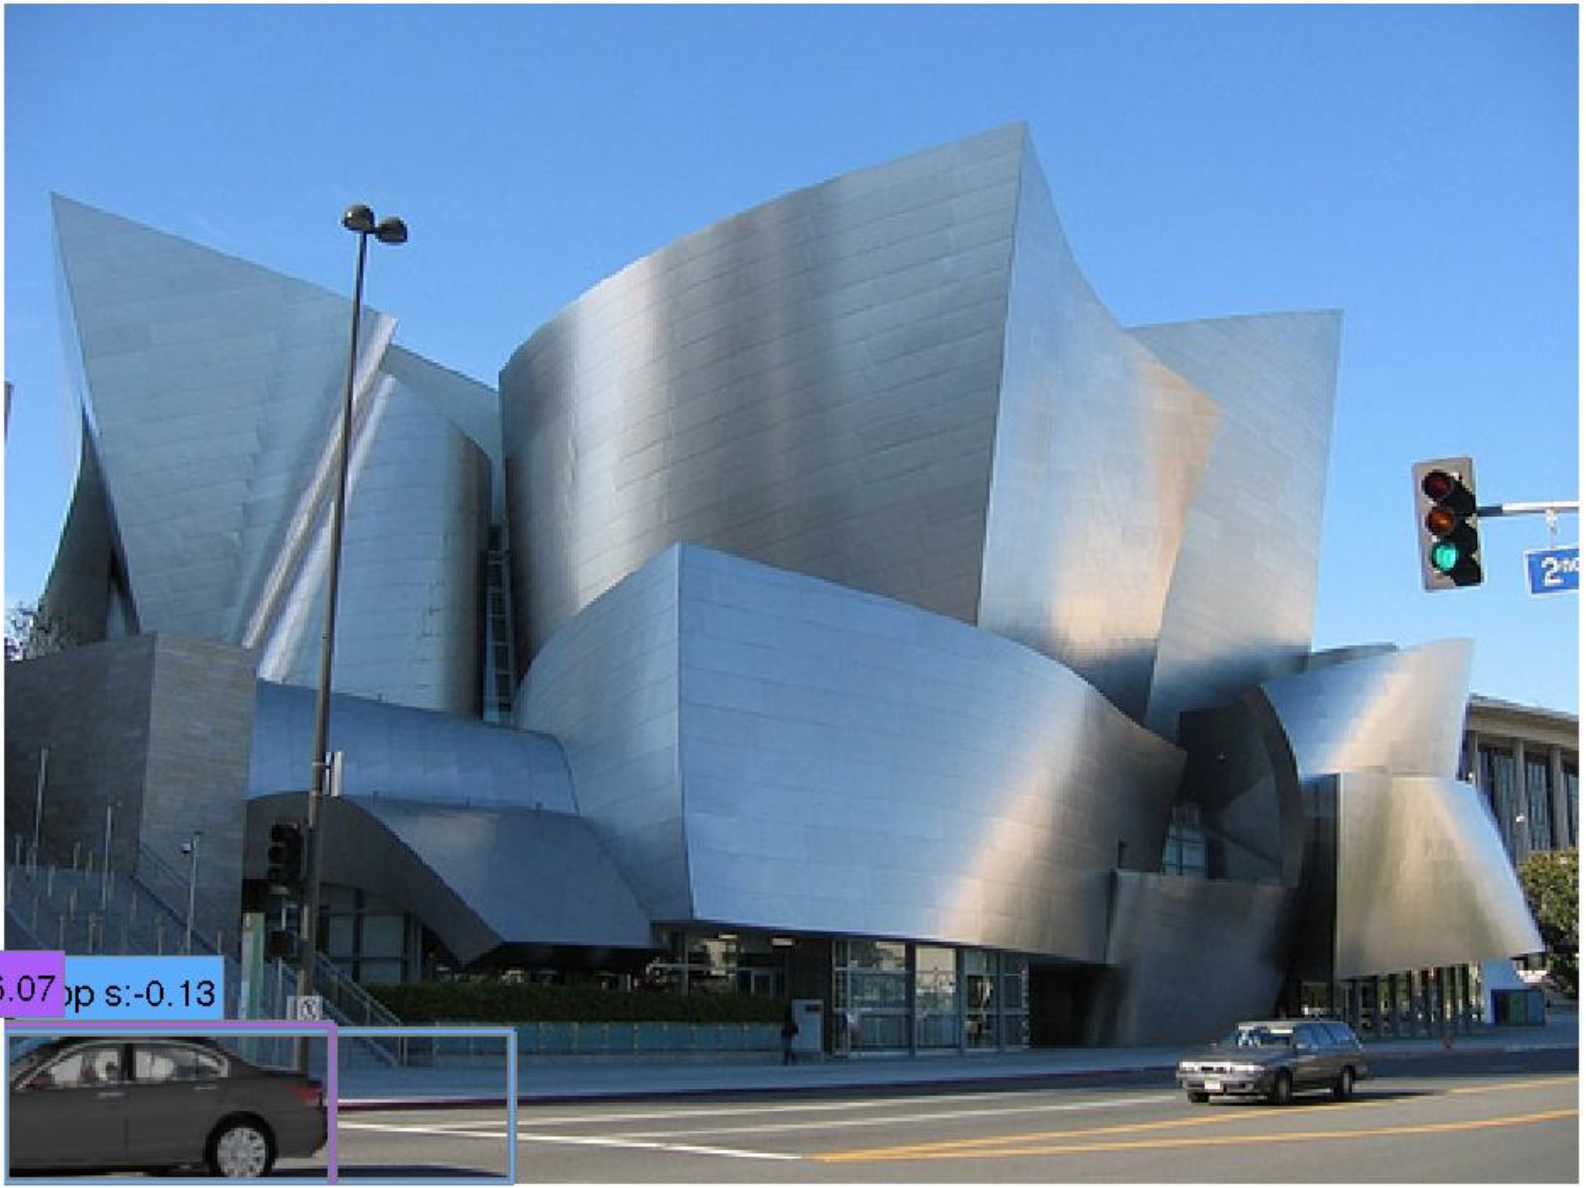
\includegraphics[width=0.24\textwidth]{car_cnn/10d.png}  \\  
        %   \hline 
        %   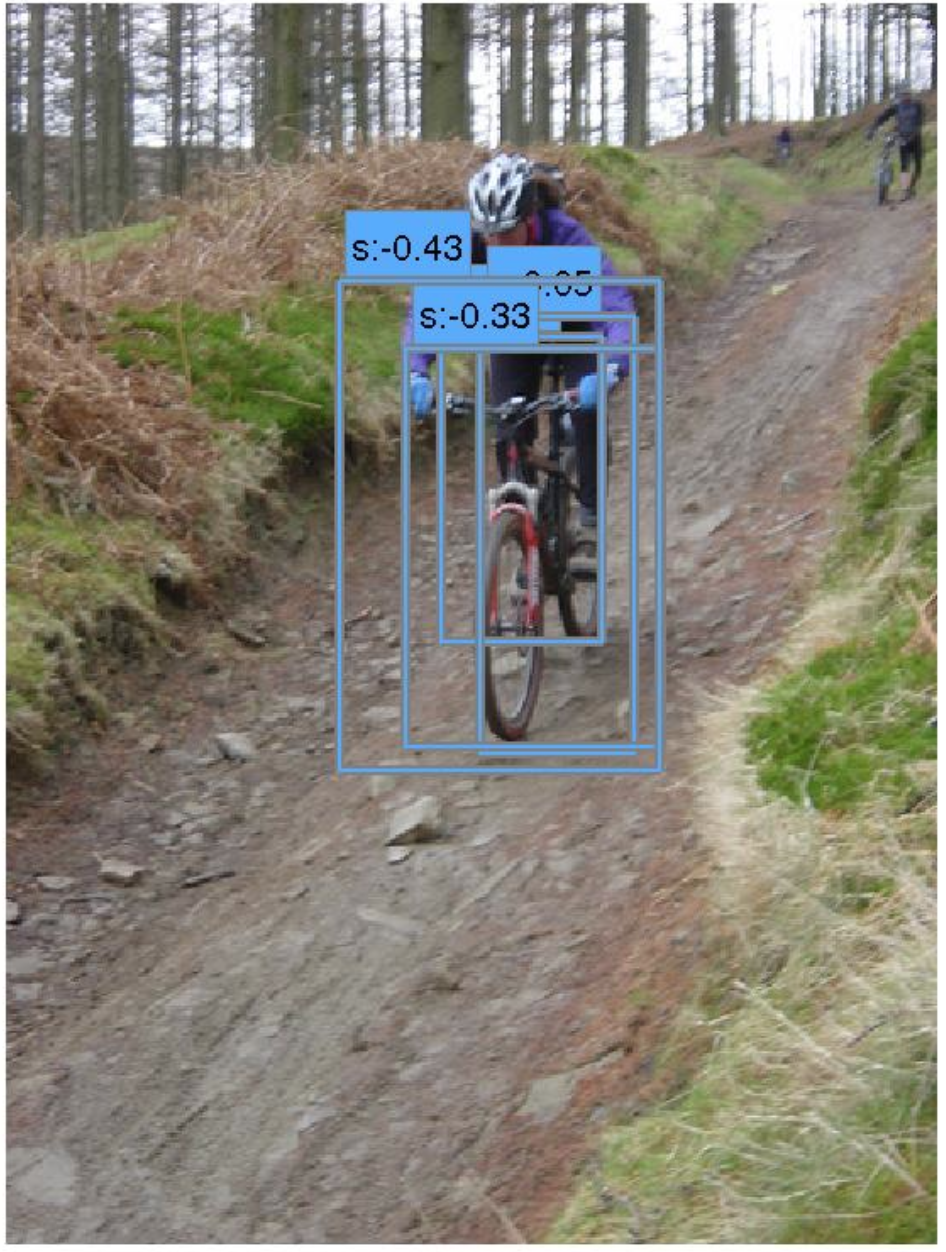
\includegraphics[width=0.24\textwidth]{bicycle_cnn/3a.png} &   
        %   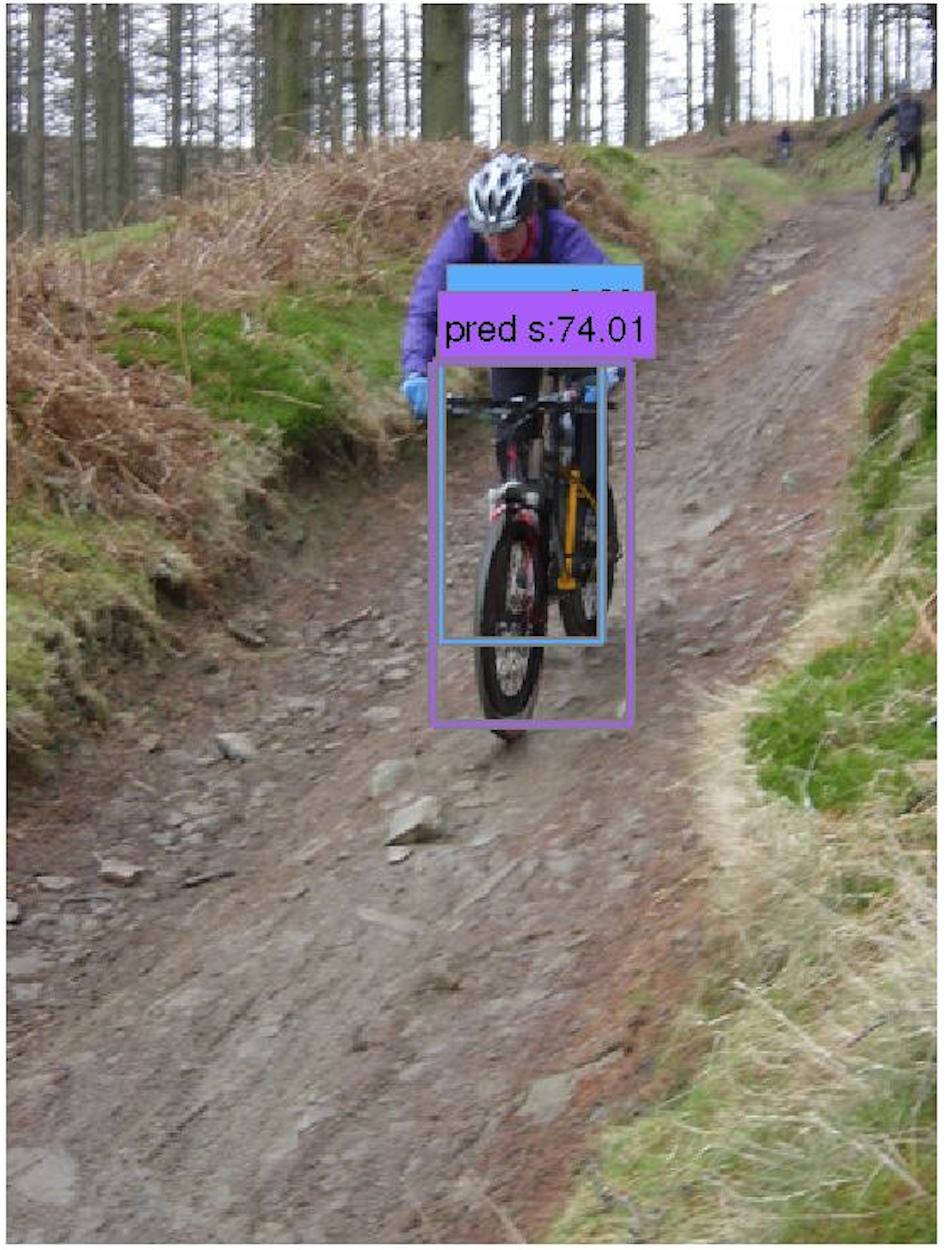
\includegraphics[width=0.24\textwidth]{bicycle_cnn/3b.png} &   
        %   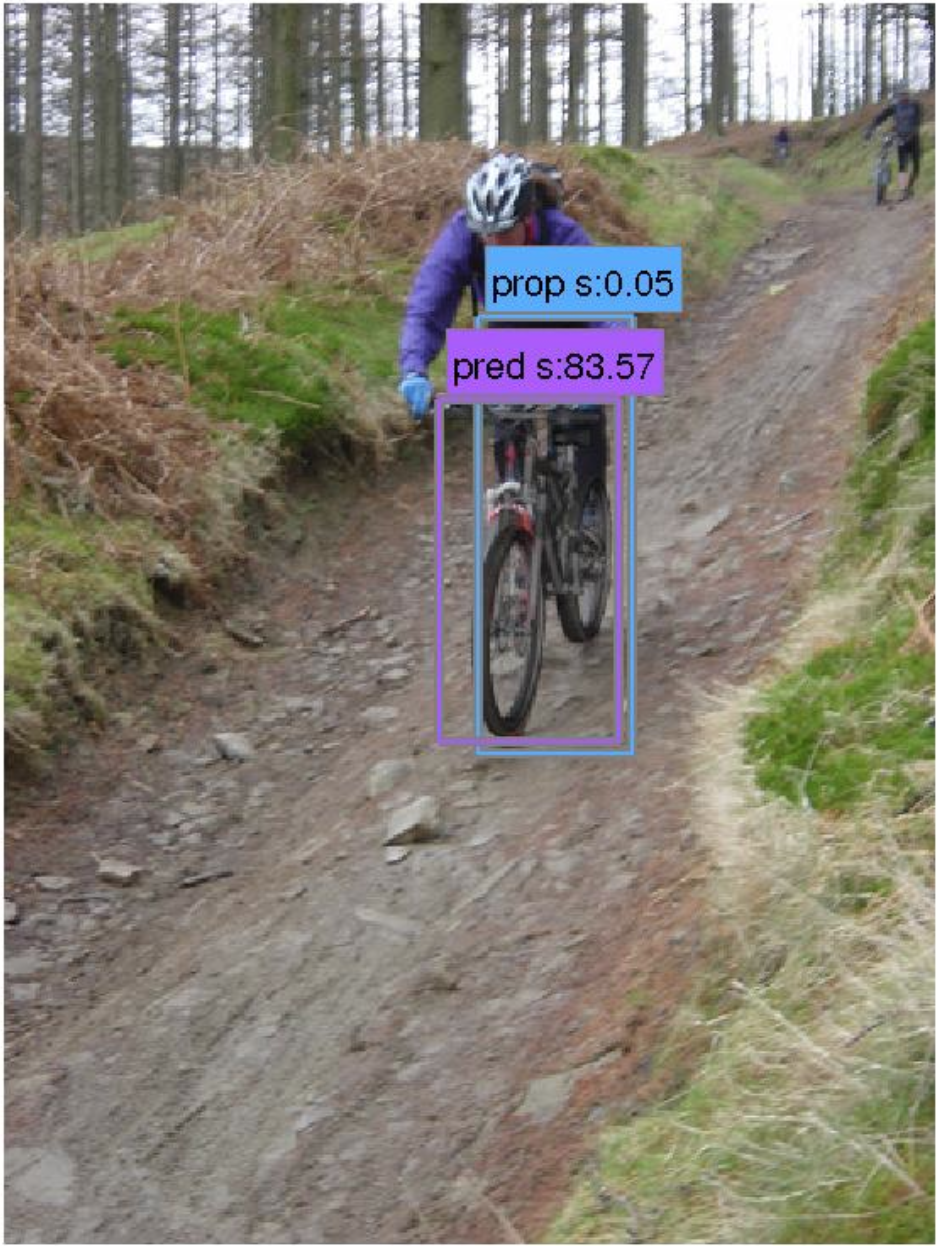
\includegraphics[width=0.24\textwidth]{bicycle_cnn/3c.png} &   
        %   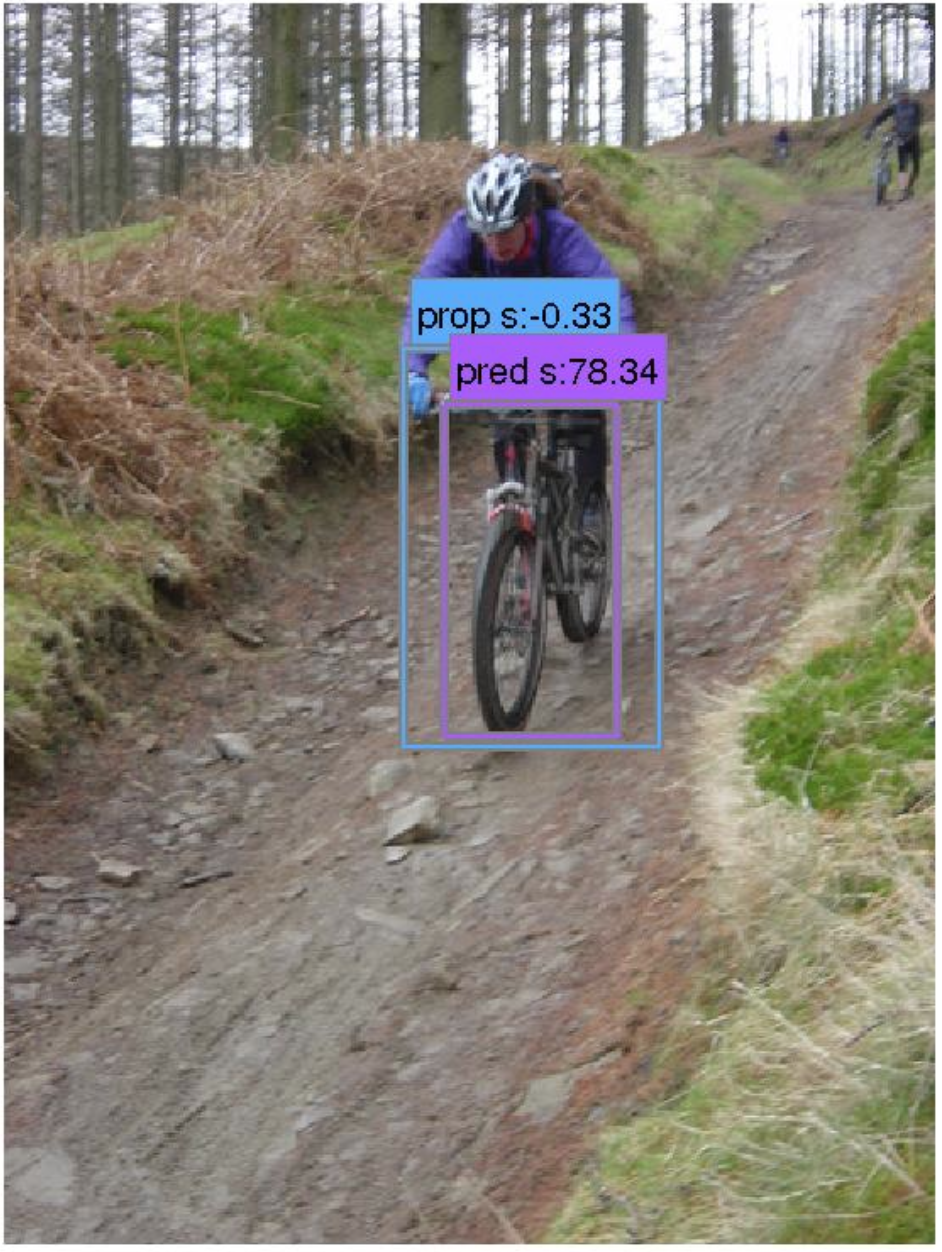
\includegraphics[width=0.24\textwidth]{bicycle_cnn/3d.png}  \\
        %
        % sorry no space
        %  \hline
        %  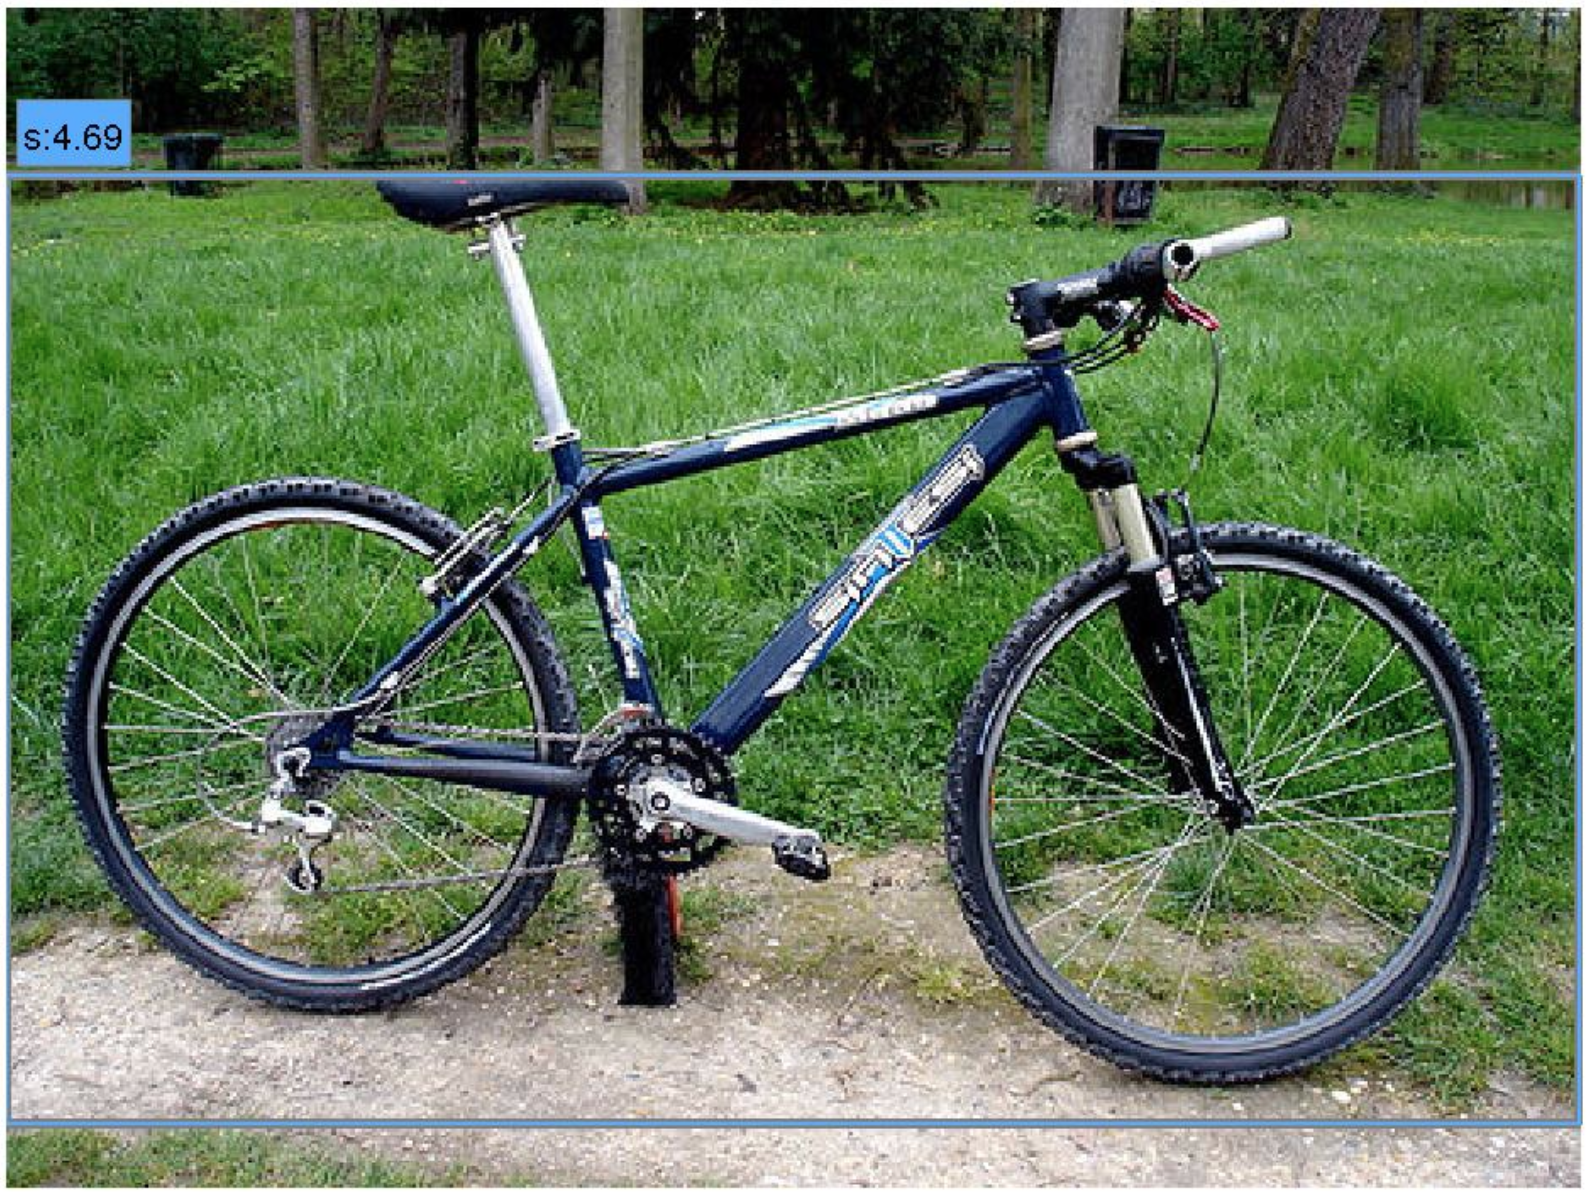
\includegraphics[width=0.24\textwidth]{bicycle_cnn/7a.png} &   
        %  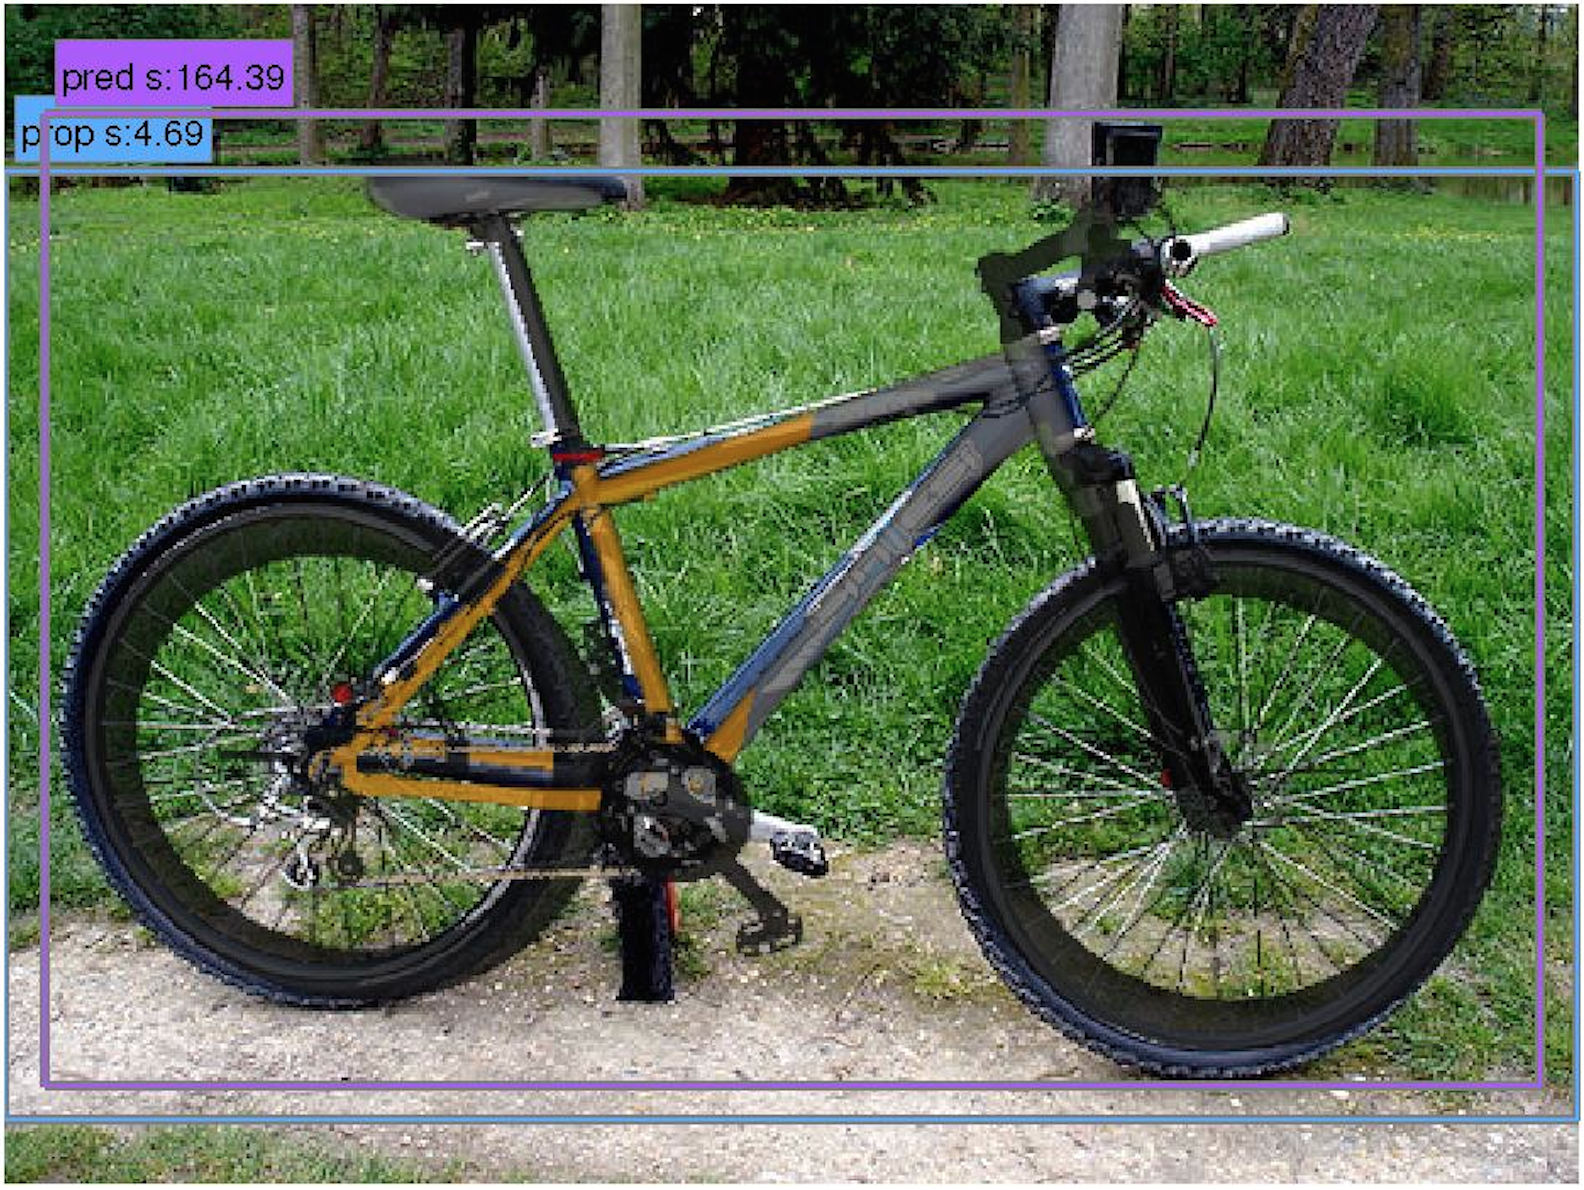
\includegraphics[width=0.24\textwidth]{bicycle_cnn/7b.png} &   
        %  &\\
          \hline
          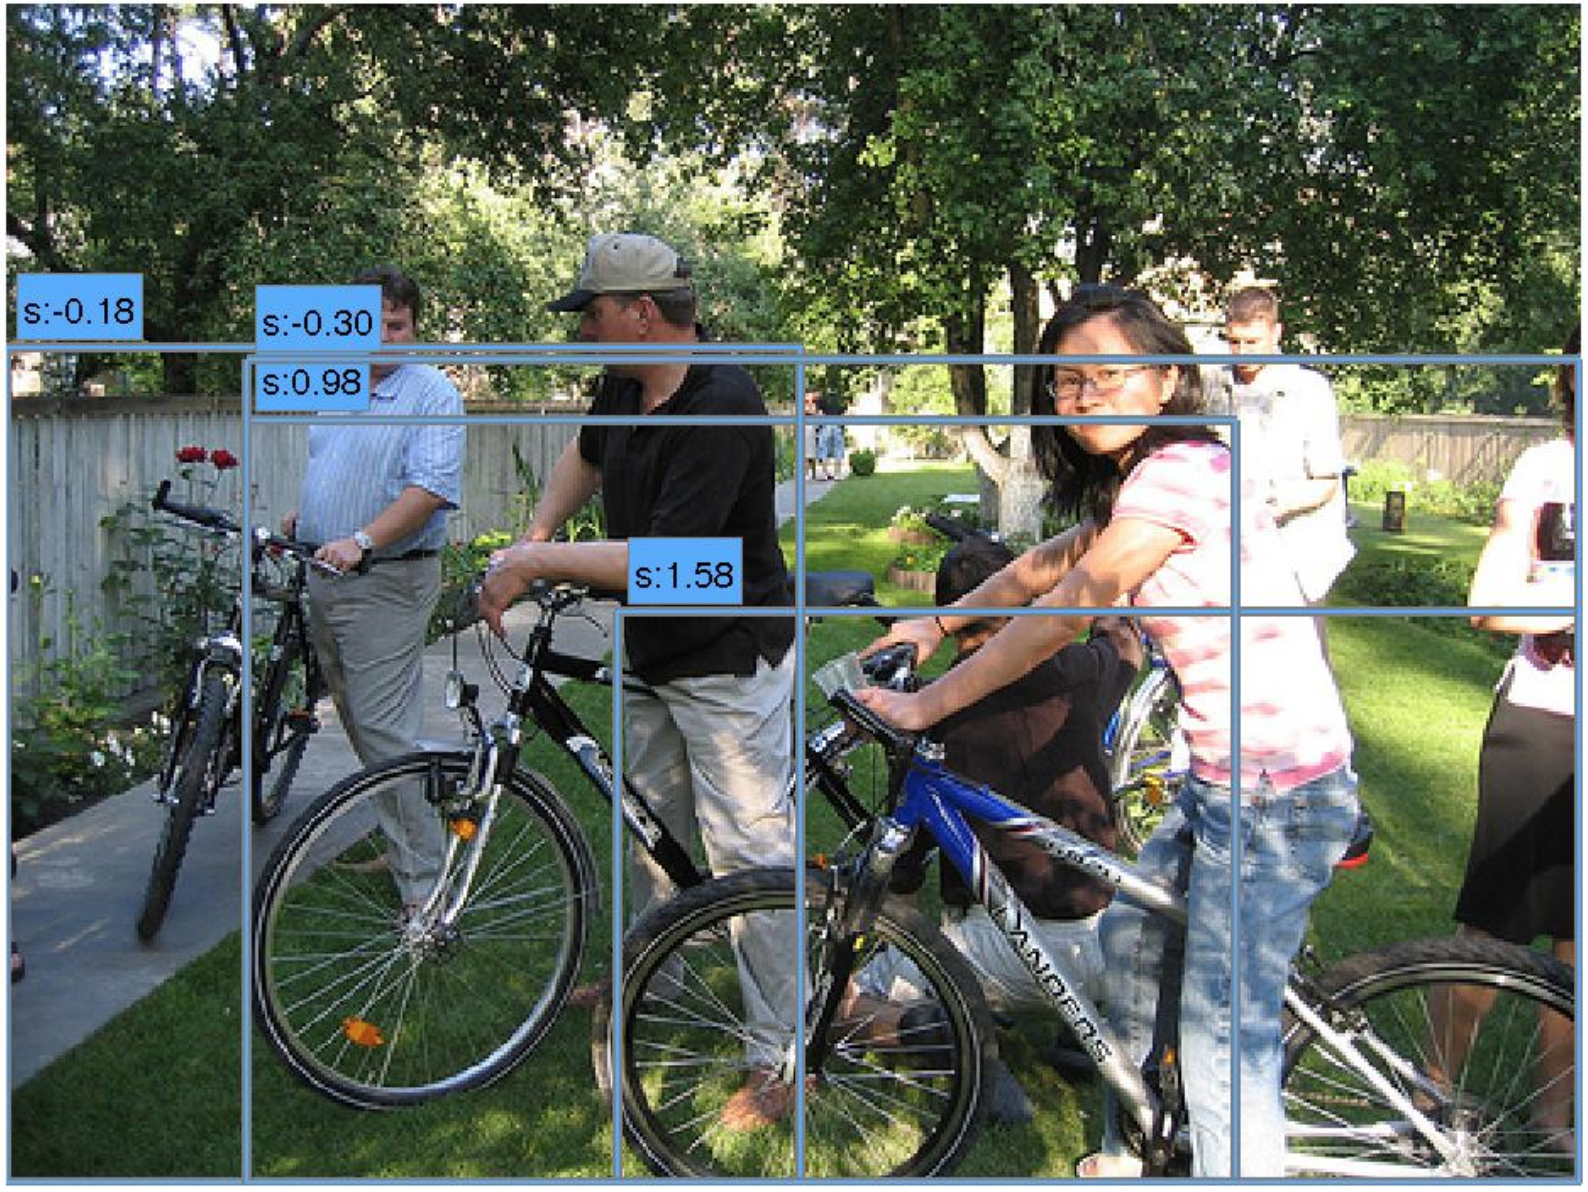
\includegraphics[width=0.24\textwidth]{bicycle_cnn/4a.png} &   
          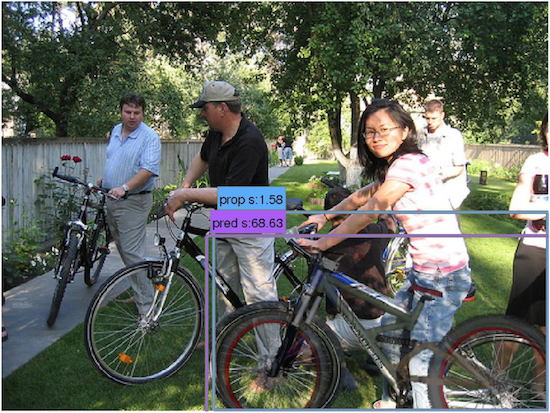
\includegraphics[width=0.24\textwidth]{bicycle_cnn/4b.png} &   
          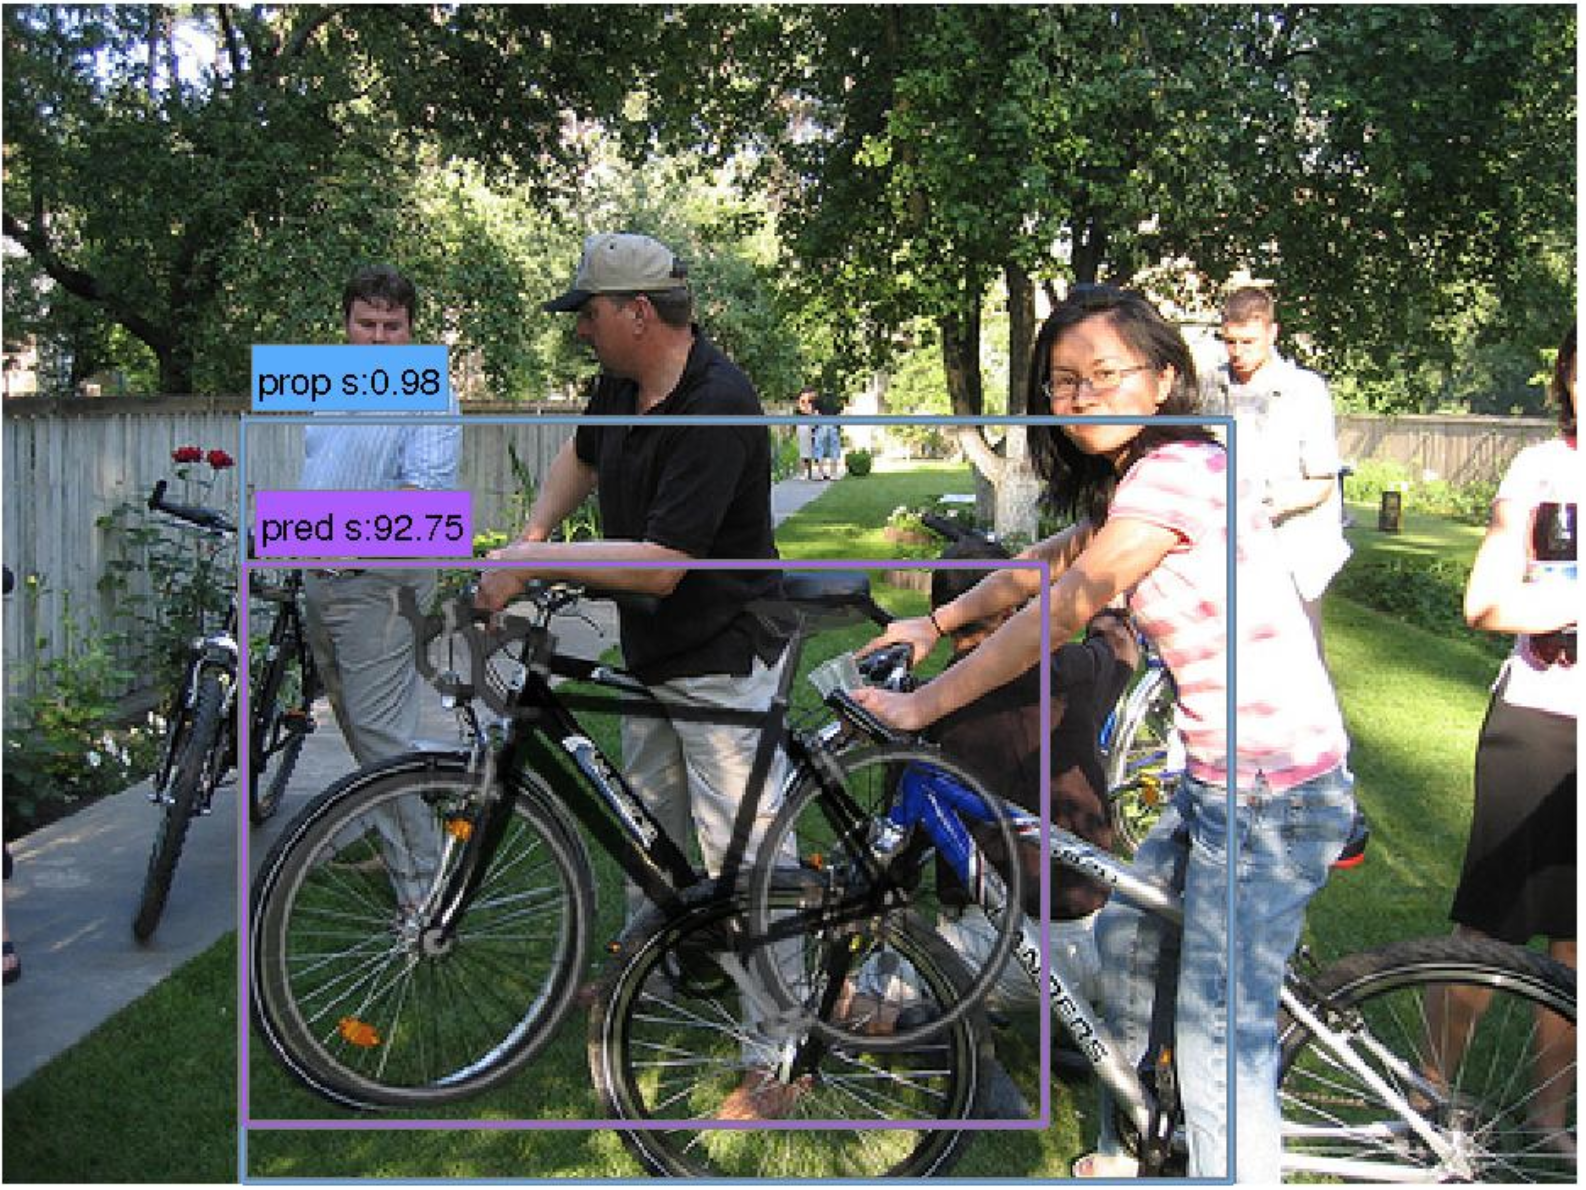
\includegraphics[width=0.24\textwidth]{bicycle_cnn/4c.png} &   
          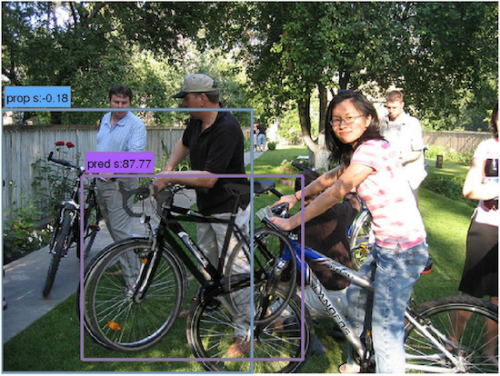
\includegraphics[width=0.24\textwidth]{bicycle_cnn/4d.png}  \\
          \hline
          CNN Proposals & \multicolumn{3}{|c|}{Our matching results on proposal bounding boxes} \\
          \hline
        \end{tabular}
        % \caption{Examples of enriched bounding boxes. Given R-CNN
        %     detection bounding boxes, our method predicted 2D-3D matching reasonably.
        %     Blue boxes are R-CNN output and purple boxes are the tightest
        %     bounding box enclosing predicted CAD model.}
        %   \label{fig:pascal12cnn}
        \end{figure}
        \vspace{-1.0em}
      \end{block}


    \end{column}
  \end{columns}
\end{frame}
\end{document}
